\documentclass[11pt,a4paper]{article}
\usepackage[utf8]{inputenc}
\usepackage[T1]{fontenc}
\usepackage{amsmath,amssymb,amsthm}
\usepackage{graphicx}
\usepackage[margin=2.5cm]{geometry}
\usepackage{hyperref}
\usepackage{xcolor}
\usepackage{booktabs}
\usepackage{authblk}
\usepackage{cite}
\usepackage{enumitem}
\hypersetup{colorlinks=true,linkcolor=blue,citecolor=blue,urlcolor=blue}

\title{\textbf{Discrete Drainage Dynamics III:\\
A Floquet Two-Step Spinor Sector and\\
Lorentz-Like Kinematic Time Dilation}}
\author[1]{Stanislas Dewavrin}
\affil[1]{Independent researcher \\ \texttt{dewavrin.iphone@gmail.com}}
\date{April 2026}

\begin{document}
\maketitle

\begin{abstract}
\noindent
\textbf{Discrete Drainage Dynamics (DDD) is an analogue-substrate
programme.} It does not contest special relativity or Lorentz
invariance: those are empirical anchors that the analogue must
reproduce in the appropriate continuum limit. We ask the
narrower, exploratory question of whether the kinematic
time-dilation factor of special relativity can arise
operationally from a discrete Floquet spinor rule inside the
toy substrate.

Papers~I and~II~\cite{paperI, paperII} treated the substrate as
a scalar reserve field $R_i \ge 0$ with first-order time
dynamics. That sector cannot
support propagating localised excitations: the rule is
diffusion-like and any initial bump spreads. Here we extend the
substrate with a two-component spinor $\psi_i \in \mathbb{C}^2$
at each node, and a Floquet two-step time evolution that
alternates a matter-hopping update~A and a gauge-twist update~B
with period $T = \tau_A + \tau_B$. Within the class of local
stateful-link rules satisfying four operational propagation
axioms (F1)--(F4), this two-step structure is selected as the
minimal two-component Pauli/Floquet representative; closing the
construction further requires a topological hypothesis~(F-twist)
that fixes the diagonal-twist normalisation
$\lambda = 1/(2\pi)$. The Floquet quasi-energy then exhibits a
band gap of magnitude $m = \lambda/T$ at the lattice
point $(\pi, 0)$, around which the dispersion is approximately
Lorentz-like, $\varepsilon^2 \approx m^2 + (c_{\rm eff}\, p)^2$
with $c_{\rm eff} = 1/T$ and explicit quartic lattice
corrections $O(\delta^4)$ in the momentum offset. Localised
wavepackets near this gap point propagate at the predicted
group velocity, and we measure operationally the kinematic
clock-rate $m/\gamma = m^2/E$ at moving packets via a
Galilean-shifted, dealiased $k$-space projection. The measured
proper-time rate matches the prediction $m/\gamma$ to better
than $1\%$ for $\gamma < 2$ (median deviation $\sim 0.3\%$ over
$\gamma \in [1, 2]$) and within $\sim 10\%$ for $\gamma < 4$,
with monotonic deviations beyond. The result is the kinematic
counterpart of the bandwidth identification of Paper~II: the
moving packet's effective clock runs at $m/\gamma$ in lab time,
measured from substrate observables without invoking Lorentz
transformation laws. We do \emph{not} derive the Lorentz group, the spatial part of
the metric, the Einstein equations, or the spinor sector
itself; their derivation is deferred to Papers~IV--VII. The
(F-twist) normalisation is the principal open problem: the
topological hypothesis fixing $\lambda = 1/(2\pi)$ closes the
construction but remains microscopically unexplained.
\end{abstract}


\noindent\fbox{\parbox{0.96\textwidth}{\small
\textbf{What this paper makes mechanically legible.}
Special relativity postulates the existence of a finite invariant
speed $c$ as an empirical input; SR/GR has no structural
explanation for \emph{why} a propagation ceiling exists, and
encodes kinematic time dilation as a metric transformation law.
\emph{This paper} forces the existence of a propagation ceiling
$c_{\rm eff} = 1/T$ from finite per-tick lattice bandwidth
(locality (L1) + (L5)), and reads the kinematic factor
$m/\gamma$ as the operational comoving phase rate of a Floquet
wavepacket --- no Lorentz transformation invoked.
\textbf{Leverage:} the \emph{existence} of $c$ becomes a
substrate consequence rather than an ad-hoc postulate, and the
SR transformation law is replaced by an operational phase-rate
measurement on a discrete medium.
}}
\bigskip


\section{Main claims and scope}
\label{sec:claims}

\paragraph{Programme positioning and analogue framing.}
Discrete Drainage Dynamics is an analogue-substrate programme;
it does not contest special relativity or Lorentz invariance.
Those are the empirical anchors the analogue must reproduce.
The aim of this paper is the narrower question of whether the
\emph{form} of the kinematic time-dilation factor can emerge
operationally from a discrete Floquet spinor rule. The result
is internal to the analogue, conditional on the axioms
(F1)--(F4) and the topological hypothesis (F-twist) introduced
in Sec.~\ref{sec:substrate}, and holds only in the continuum
limit and for the specific spinor sector adopted. Any deviation
of the analogue from special relativity at the level of
measured tests is a falsifier of the analogue, not of SR.


This paper introduces a structurally new sector of the substrate
beyond the scalar reserve of Papers~I and~II, and uses it to
recover a Lorentz-like kinematic clock-rate relation
$\omega_{\rm comov} = m/\gamma$ at moving wavepackets.

\begin{enumerate}
\item \textbf{Spinor sector.} The substrate carries, in addition
to the scalar reserve $R_i$ of Paper~I, a two-component
$\mathbb{C}^2$ spinor field $\psi_i = (a_i, b_i)^\top$ at each
node, evolving under a Floquet two-step rule. The spinor sector
is decoupled from the scalar reserve in this paper; coupling is
deferred to Paper~VII.

\item \textbf{Lorentz-like dispersion.} The Floquet quasi-energy
of the spinor sector exhibits a band gap of magnitude
$m = \lambda/T$ at the lattice momentum $(\pi, 0)$, with
$\lambda = 1/(2\pi)$ from (F-twist) and $T = \tau_A + \tau_B$.
Near this gap point, the dispersion is approximately
\begin{equation}
E^2 \;\approx\; m^2 + c_{\rm eff}^2\, p^2 + O(\delta^4),
\qquad c_{\rm eff} = 1/T,
\label{eq:lorentz_dispersion_claim}
\end{equation}
where $p = k - k_0$ is the momentum offset from the gap and the
$O(\delta^4)$ correction is computed analytically in
Sec.~\ref{sec:lattice}. Excitations near the gap are massive,
relativistic, and propagate at the group velocity
$v_g = \partial E/\partial p$.

\item \textbf{Operational kinematic clock identification.} For a
localised wavepacket centred at momentum $p$ with energy $E(p)$
and group velocity $v_g(p)$, the dealiased Galilean-shifted
projection
\[
A_{\rm comov}(t) \;=\; \langle k_0 | \psi(t) \rangle
\cdot \exp(-i\,p \cdot v_g\, t)
\]
has a phase rate equal to $E - p \cdot v_g = m^2/E$ in the
continuum Lorentz limit. This is the kinematic counterpart of
the bandwidth identification of Paper~II: the operational
\emph{proper-time rate} of the moving packet is $m/\gamma$.

\item \textbf{Numerical verification.} The measured proper-time
rate matches $m/\gamma$ to better than $1\%$ for $\gamma < 2$
(with relative deviations in $[0.01\%, 1.3\%]$, median
$\sim 0.3\%$) and remains within $\sim 10\%$ up to $\gamma = 4$.
Beyond $\gamma \sim 5$, lattice corrections to Lorentz become
significant; we quantify them analytically (quartic in the
momentum offset, Sec.~\ref{sec:lattice}) as a structural
prediction of the discrete substrate.
\end{enumerate}

\textbf{Limitations and scope.}

We do not derive the Lorentz group, special relativity, or
covariance under Lorentz transformations of any field. Within
the candidate spinor sector adopted in Sec.~\ref{sec:substrate},
we recover the operational relation $\omega_{\rm comov} =
m/\gamma$ in the continuum limit of the lattice rule. We do not
derive the spatial part of the metric, the photon sector, or
the Einstein field equations. The derivation in
Sec.~\ref{sec:floquet-axiomatic} establishes that the Floquet
two-step structure with a 2-component Pauli spinor is the
minimal representative within the class of local stateful-link
substrates satisfying four operational axioms (F1)--(F4).
However, the diagonal-twist normalisation $\lambda = 1/(2\pi)$
is not derived from those axioms: it is adopted as a
\emph{topological hypothesis}~(F-twist) on the unit-flux
quantisation of the diagonal-twist sector, and constitutes the
principal open problem of the construction. We do not address
the coupling between the spinor and the scalar sector: in this
paper they are independent. The coupling and any related
conservation laws are deferred to Paper~VII; the schematic
combined gravitational--kinematic factor of
Sec.~\ref{sec:bridge} is a \emph{conjecture} for that paper,
not a verified result of the present one.

\subsection*{Motivation and significance}
\addcontentsline{toc}{subsection}{Motivation and significance}

Special relativity is one of the most mysterious empirical facts of
physics for everyday intuition: clocks slow with motion, lengths
contract, mass is convertible into energy via $E = mc^2$, and the
speed of light is the same for every inertial observer. In standard
physics, Lorentz invariance is an \emph{input postulate}: the
Minkowski metric and the universal $c$ are taken as given, and the
kinematic consequences (time dilation, length contraction) follow
mathematically. The framework is descriptive, not derivative.

This paper proposes a different reading of the kinematic phenomena.
The substrate of Paper~I is supplemented with a Floquet two-step
spinor sector --- the same substrate, with two interleaved tick
phases (A and B) and a two-component spinor $\psi$ on each node.
This sector supports propagating localised excitations whose
band-structure is that of a 3D Weyl semimetal. Near the Weyl points,
the dispersion is linear and isotropic: $\omega(\mathbf{k}) =
v_g\,|\mathbf{k}|$. An operational clock measurement on these
excitations --- comoving with the wavepacket --- yields a
\emph{kinematic} clock-rate dependence that matches the Lorentz form
$\sqrt{1 - v^2/c^2}$ at the percent level for $v < 0.5\,c$.

This is not a derivation of full Lorentz invariance: the substrate
breaks exact Lorentz at high momenta where lattice anisotropy
dominates, and the spinor sector is a structural extension beyond the
scalar reserve of Paper~I. But it shifts the kinematic mystery: in
DDD, time dilation is not a consequence of postulated Lorentz
invariance, it is an operational consequence of how propagating
excitations are clocked on a discrete substrate. The deeper question
--- why the substrate admits the Floquet 2-step structure --- is the
principal open question of this paper.




\paragraph{Which mystery does this paper address?}
Per SERIES\_FEEDBACK §0.bis, this paper targets:

\begin{itemize}
\item \textbf{Mystery~\#1 (the speed-of-light ceiling).} The
Floquet two-step rule has a finite group-velocity ceiling
$c_{\rm eff} = 1/T$ set by the substrate's tick period. We
identify this ceiling as the analogue counterpart of the
empirical $c$. The paper does not derive the CODATA value of
$c$ in physical units; it derives the existence of the ceiling
from finite per-tick bandwidth.
\item \textbf{Mystery~\#5 (operational origin of inertia and
the kinematic clock-rate).} SR/GR encode both through metric
postulates. We ask whether a kinematic time-dilation factor of
Lorentz-like form ($m/\gamma$) arises operationally from a
discrete Floquet spinor rule on a lattice. The answer offered
here: under axioms (F1)--(F4) and the topological hypothesis
(F-twist), the analogue's comoving phase rate matches the
form of $m/\gamma$ in the continuum limit near a band gap.
The microscopic origin of (F-twist) (and hence the value of
$\lambda = 1/(2\pi)$) is open and is the principal
$why$-question this paper does \emph{not} resolve.
\end{itemize}

\paragraph{Distinctive contribution and ontological reading.}
Special relativity postulates Lorentz invariance and the
existence of a finite invariant speed $c$. Within SR/GR, there
is no structural explanation of \emph{why} $c$ exists, or why
it has the role of a propagation limit; Lorentz transformations
are taken as postulates, not derived. Likewise, kinematic time
dilation $\sqrt{1 - v^2/c^2}$ follows from the metric's
indefinite signature, not from a mechanism. These are the
distinctive points where the present paper's analogue
contributes:

\begin{enumerate}
\item \textbf{Structural origin of the speed-of-light ceiling.}
SR/GR introduces $c$ as an empirical postulate; there is no
mechanical answer in the standard formalism to ``why does a
finite propagation ceiling exist at all?''. In the analogue,
the discrete tick $\tau$ and the per-link bandwidth $\alpha$
together force the existence of a bounded group velocity
$c_{\rm eff} = 1/T$ \emph{by construction}: information cannot
cross more than one lattice link per tick, hence cannot
propagate faster than $c_{\rm eff}$. \textbf{The existence of a
finite speed-ceiling is therefore not postulated in DDD; it is
a structural consequence of locality (L1) and finite per-tick
bandwidth (L5).} Identification with the empirical CODATA $c$
remains a calibration; the \emph{existence} of the ceiling does
not.

\item \textbf{Operational origin of the kinematic time-dilation
factor.} In SR, $m/\gamma$ is a transformation law: an inertial
observer infers it via the Lorentz boost. Here, $m/\gamma$ is
the \emph{operationally measurable} comoving phase rate of a
moving wavepacket, $\omega_{\rm comov} = E - p\,v_g = m^2/E$.
No Lorentz transformation is invoked at any stage; the
analogue produces the same factor as a substrate-level rate.
\textbf{This displaces a transformation-law fact into a
phase-rate measurement on a discrete medium.}

\item \textbf{Mechanical reading of inertia.} In GR/SR,
inertia is encoded geometrically (the metric pairs energy and
momentum). In the analogue, a faster-moving wavepacket has its
lab-frame energy split between rest mass and kinetic
momentum, and its comoving phase rate is correspondingly
suppressed. The bandwidth interpretation reads ``moving
clocks tick slow'' as ``moving packets have less bandwidth
available for their internal phase, the rest of which is
spent on translating the centroid''.
\end{enumerate}

\paragraph{What is calibrated and what is genuinely
explanatory.} The numerical value of $\lambda = 1/(2\pi)$ via
(F-twist), and the conversion of $T$ into the empirical $c$,
are \emph{calibrated} (see calibration ledger). The
\emph{existence} of a propagation ceiling, the \emph{form} of
the kinematic factor $m/\gamma$, and the operational
\emph{mechanism} of the comoving phase rate are all
substrate-level consequences. The distinctive contribution is
the displacement of the foundational SR postulates (existence
of $c$, the form of time dilation) into substrate-level
statements that are individually testable.



\section{Physical picture in plain words}
\label{sec:picture}

Picture each node of the substrate as a small arrow in two
dimensions. Not an arrow in physical space --- an arrow in an
abstract internal space. It can point anywhere on a unit
circle, and it has a phase: the angle that fixes where on the
circle it is currently pointing. That arrow is the spinor.

Picture each link between two neighbouring nodes not as a pipe
that carries flow, but as a turnstile that imposes a small
twist when the arrow at one end is communicated to the arrow
at the other. The twist is not free; it is fixed by the
geometry of the lattice. On axis-aligned links the twist is one
of three standard rotations; on diagonal links the twist
includes a small irrational $\lambda = 1/(2\pi)$. The
arrows-and-twists are the entire substrate as far as this
paper is concerned.

Now picture the rule. The arrows are not driven by an external
clock; they update themselves. At each tick of substrate time,
two things happen, in order: first the arrows at the nodes
change a little, listening to the arrows on the neighbours
through the link twists (the \emph{node-update}); then the
link twists themselves slide a little, adjusting to the new
arrow directions (the \emph{link-update}). Tick complete. The
two sub-events alternate. Alternation is the natural choice, because while
the link twist is being adjusted, the arrows must hold still
for the twist to know what it is registering, and while the
arrows are being updated, the link twists must hold still for
the arrows to know what they are listening to. One clean way to preserve locality with stateful links is
strict alternation of the two; we adopt this construction here.

What about a particle? A particle is not a thing one places on
a node. A particle is a coherent pattern across many arrows --- a
``packet'' --- in which the arrows rotate together at a common
phase rate, with a smooth envelope of amplitude that is
non-zero in some region and decays to zero outside. A particle
at rest is a packet whose centroid does not move; the
constituent arrows just rotate in place at a steady rate. A
particle in motion is a packet whose centroid drifts in some
direction; the constituent arrows still rotate, but as the
packet drifts, an observer who keeps watching the same lattice
site sees the packet pass through, and the arrow at that site
goes through a more complicated pattern --- amplitude that
rises and falls, with phase that is twisting at a faster rate
than the rest packet.

The mass of the particle is set by how fast the arrows rotate
when the packet is at rest. The momentum of the particle is set
by the wavelength over which the smooth envelope's phase
twists across the lattice: short wavelength, high momentum.
The maximum speed at which a packet can drift is fixed by the
substrate; we call it $c_{\rm eff}$. No packet can drift
faster, because beyond that speed the lattice rule has nowhere
to put the next site.

What is then the kinematic time dilation of a moving packet?
Watch the packet from outside, in lab time. A rest packet's
arrow rotates at rate $m$ (its mass). A moving packet's arrow
rotates faster --- at rate $E$, where $E^2 = m^2 +
(c_{\rm eff}\, p)^2$. But that is the lab observer's clock
reading. If we instead ask what \emph{the packet itself
experiences} --- the rate at which the substrate updates
relative to the packet's smooth-envelope frame, after
subtracting the trivial drift of its centroid --- we find a
rate that decreases with speed: it equals $m^2/E = m/\gamma$.
The packet's own clock, measured operationally on the substrate
without invoking any Lorentz transformation, runs slow by the
factor $1/\gamma$.

This is the kinematic counterpart of Paper~II's bandwidth
identification. There, the local clock rate of a static node in
a gravitational well was the locally available reserve $R/R_0$.
Here, the local clock rate at a moving spinor packet is its
own substrate-update rate as seen from its smooth-envelope
frame: $m/\gamma$. The mechanism is different (gravitational
deficit vs. kinematic motion), but the operational logic is
the same: read the rate of activity from the substrate, and
identify it with the rate of effective proper time.

The body of the paper makes this precise. The first task is to
write down the rule that produces this picture, and to motivate
why the rule must take the form it does.

\section{Beyond the scalar reserve: the Floquet two-step spinor sector}
\label{sec:substrate}

\subsection{Axiomatic derivation of the Floquet two-step spinor structure}
\label{sec:floquet-axiomatic}

The Floquet two-step spinor rule introduced in this section is
the central structural ingredient of the kinematic time-dilation
result. The motivation given in the literature for such rules is
usually post hoc: ``the two-step Floquet structure conveniently
produces a Weyl-like dispersion that supports propagating
excitations.'' That is a logic of compatibility, not derivation,
and it leaves the rule open to the obvious peer-review objection:
\emph{any local rule with the right low-energy effective theory
would also be compatible}. This subsection closes that gap by
deriving the rule structure uniquely from four operational
axioms on a local update that supports propagating excitations,
before any appeal to Lorentz phenomenology or Weyl-semimetal
analogy.

\paragraph{The four propagation axioms.}
Let the substrate consist of nodes carrying local amplitudes
and links carrying independent state (phases or twist
holonomies, distinct from the node amplitudes). Within this
class of substrates, the local update rule is constrained by
four operational axioms.

\begin{enumerate}[label=(F\arabic*)]
\item \textbf{Sub-tick causal locality for stateful links.}
We restrict the class of rules to those decomposed into
elementary local operations in which each operation reads a
fixed neighbouring state and writes the corresponding local
update. (A globally synchronous update that reads all variables
at $t$ and writes all variables at $t+\Delta t$ is admitted at
the level of the global tick but, when decomposed into
elementary operations, falls outside this class for stateful
links.) Within this class, the minimal non-self-referential
update on a graph where both nodes and links carry independent
dynamical state is an alternation: nodes update with link state
held fixed, then links update with node state held fixed. The
rule is two-step over one tick. This axiom does \emph{not}
exclude synchronous-cellular-automaton updates of stateless
links; it characterises the minimal sequentially-causal
decomposition for the stateful-link case.

\smallskip
\noindent\emph{Brief existence/uniqueness argument.}
Any sub-tick that simultaneously reads and writes both the
node variable on a vertex and the link variable on an
incident edge requires a precedence convention to resolve which
value is supplied to which. Adopting that convention is
logically equivalent to splitting the sub-tick into two halves,
one reading the link state into the node and the other reading
the node state into the link --- i.e., the alternation written
above. Conversely, any non-alternating decomposition either
allows a freshly-rewritten variable to feed the same sub-tick
(violating no-self-reference) or duplicates state by buffering
both old and new values (which is the alternation in disguise,
implemented by an extra read--write pass). The two-step
node--link split is therefore the minimal non-trivial
sequentially-causal decomposition compatible with the stated
class.

\item \textbf{Per-sub-tick unitarity.}
Each sub-tick is a norm-preserving operation on the global
amplitude state. Equivalently, the per-sub-tick operator is
unitary on the local Hilbert space at each node and at each
link. This guarantees exact conservation of total amplitude
under repeated cycles and is the analogue of internal
conservation~(L2) of Paper~II for a complex amplitude sector.

\item \textbf{Minimal complex amplitude carrying both
orientation and phase.}
The local amplitude at each node must carry: (i) a phase, to
encode the position in its internal oscillation cycle; and
(ii) an orientation, to distinguish forward and backward
propagation directions. One complex component carries phase
but cannot encode orientation independently of phase. Two
complex components is the minimum sufficient: the relative
phase between components encodes orientation, while the
overall phase encodes the cycle position. Three or more
complex components would introduce additional bands without
enriching the local orientation structure, and are excluded
by minimality.

\item \textbf{First-order reversible propagation.}
A closed, reversible propagating sector must have a low-energy
generator whose leading spatial term is first order in
momentum. On a lattice, locality together with parity pairing
makes the minimal odd kinetic term proportional to $\sin(k_a)$
in the momentum representation. With the two-component minimal
internal space of (F3), the Clifford/Pauli algebra is the
minimal way to combine independent first-order spatial
directions into a positive low-energy dispersion: the natural
minimal kinetic structure is
\[
H_{\rm kin}(k) \;=\; \sin(k_x)\,\sigma_x + \sin(k_y)\,\sigma_y ,
\]
with the third Pauli generator $\sigma_z$ available to open the
mass gap. The Lorentz-like dispersion $E^2 = m^2 + (cp)^2$ at
the gap closure is then a \emph{consequence} of this minimal
first-order kinetic structure, not an additional input.
\end{enumerate}

\paragraph{What (F1)--(F4) minimally select.}
Axioms (F1)--(F4) fix the structural ingredients of the rule:
\emph{sequential alternation in the stateful-link case} (from F1),
\emph{per-sub-tick unitarity} (from F2), \emph{a 2-component
complex spinor at each node} (from F3), and \emph{first-order
reversible propagation realised via Pauli kinetic operators with
$\sin(k_a)$ momentum-space form} (from F4). Axioms (F1)--(F4)
do \emph{not} prove uniqueness among all possible discrete-time
quantum walks: the class of split-step Floquet walks contains
several inequivalent realisations that are nevertheless
low-energy-equivalent. What (F1)--(F4) select is the
\emph{minimal two-component Pauli/Floquet representative} of
the local reversible propagation class, with the rule structure
of Eqs.~(\ref{eq:floquet_cycle})--(\ref{eq:HB}) below as one
representative, modulo a single scalar parameter~$\lambda$
controlling the diagonal twist density. Other representatives
exist within the class; they are either related by local
unitary changes of basis, add redundant bands, or modify the
UV corrections while preserving the same low-energy Dirac form.

\paragraph{Comparison with Wilson and Kogut--Susskind.}
Wilson fermions~\cite{wilson1974} and Kogut--Susskind staggered
fermions~\cite{kogut1975} are not the representatives adopted
here because they implement the continuum Dirac structure
through different lattice mechanisms (Wilson term as
momentum-dependent mass; staggered as sublattice-doubling
without minimal Clifford structure). They are useful comparators
and provide independent routes to the same Dirac-like
low-energy theory; they lie outside the minimal stateful-link
Floquet class defined by (F1)--(F4) rather than being violators
of those axioms in any pejorative sense. The choice of the
present minimal-representative class is one of architectural
economy of principle, not a claim of exclusion of well-established
constructions.

\paragraph{The substantive remaining hypothesis: topological
twist normalisation.}
Axioms (F1)--(F4) leave the diagonal-twist constant $\lambda$
in $H_B$ undetermined. A fully closed construction further
requires a normalisation choice for the diagonal-twist sector.
We adopt one such choice as a \emph{topological hypothesis}
rather than as an additional operational axiom:

\begin{description}
\item[(F-twist, hypothesis) Single $2\pi$ winding per plaquette
diagonal.]
The diagonal twist density on the lattice is normalised to
exactly one $2\pi$ phase winding per unit area of plaquette
diagonal, equivalent to the unit flux-quantum normalisation of
the diagonal-twist sector. We motivate this choice as the
topologically smallest non-trivial U(1) holonomy structure
compatible with the bipartite-sublattice structure forced by
(F3), but emphasise that it is a \emph{hypothesis} on the
substrate, not derived from substrate microphysics.
\end{description}

(F-twist) is the substantive hypothesis that closes the
construction and determines $\lambda$ uniquely.
\textbf{Calibration-vs-derivation status (per
SERIES\_FEEDBACK §0.ter).} Within the present paper,
$\lambda = 1/(2\pi)$ is adopted as a \emph{topological-minimality
hypothesis}, not a calibrated input fitted against an empirical
quantity --- there is no SM/GR observable or CODATA constant
whose value pins $\lambda$ directly. Equivalently: the
\emph{form} $m = \lambda/T$ of the gap mass is a substrate
consequence of (F1)--(F4)+(F-twist); the \emph{value} of
$\lambda$ is held by the topological hypothesis pending a
microscopic derivation. Future work that derives $\lambda$ from
a substrate-graph topological invariant or a Chern--Simons
closure condition would convert this hypothesis into a
derivation per the §0.ter trajectory. It is the
analogue of (L4) for the present paper: it is what an attacker
of the construction must engage with rather than the structural
ingredients themselves. The four propagation axioms (F1)--(F4)
are operational requirements of any local rule supporting
propagating excitations on a graph with stateful links;
(F-twist) is the topological normalisation that selects which
member of the (F1)--(F4) class the substrate realises.
Throughout, we use ``axiom'' for (F1)--(F4), which we regard as
operational requirements, and ``hypothesis'' for (F-twist), to
flag that its origin is the principal open problem of the
construction (Sec.~\ref{sec:open}). The kinematic result
$\omega_{\rm comov} = m/\gamma$ derived below is therefore
\emph{conditional} on (F-twist): the gap mass $m = \lambda/T$
depends linearly on $\lambda$, so a different topological
normalisation would shift the mass scale and all $\gamma$-dependent
predictions.

\paragraph{Where each axiom can be attacked.}
\begin{itemize}
\item Attacking (F1) (sub-tick causal locality) means
admitting elementary operations that read a variable being
simultaneously rewritten in the same sub-tick; this is allowed
for stateless links (synchronous cellular automaton) but
introduces unresolved precedence questions for stateful links.
A different framework would either return to stateless links
(losing the propagating sector) or introduce a precedence rule
that effectively reintroduces an alternation.
\item Attacking (F2) (per-sub-tick unitarity) means allowing
non-conservative amplitude evolution; this is incompatible with
the closed-system substrate of Papers~I--II.
\item Attacking (F3) (minimal complex amplitude) requires
positing either a real-valued amplitude (which cannot carry
phase) or a higher-rank multiplet (which generates redundant
bands without enriching the orientation structure); both
introduce structural elements beyond the minimum.
\item Attacking (F4) (first-order reversible propagation)
amounts to giving up first-order reversible propagation in
favour of either diffusive (parabolic) low-energy behaviour or
higher-order kinetic terms with no Lorentz-like limit; this
is incompatible with the kinematic time-dilation target of the
present paper.
\item Attacking (F-twist) (single $2\pi$ winding per plaquette
diagonal) is the substantive choice. It is not an operational
requirement; it is a topological normalisation that fixes
$\lambda$ and through it the gap mass $m = \lambda/T = 1/(4\pi)$.
A microscopic explanation of why the diagonal twist sector
selects unit flux quantisation would close the remaining gap.
\end{itemize}

This axiomatic framing replaces the previous compatibility
logic ``two-step Floquet $\Rightarrow$ Weyl-like dispersion'' by
the more structured statement ``locality + unitarity + minimal
complex amplitude + linear kinetic dispersion select the
two-step Floquet structure with 2-component Pauli spinor as the
minimal representative; the topological twist-normalisation
\emph{hypothesis} $\lambda = 1/(2\pi)$ then closes the
construction.'' The hypothesis status of (F-twist) is
foregrounded in the abstract and elevated to the principal open
problem in Sec.~\ref{sec:open}.

% =====================================================================
\subsection{Why we need more than the scalar rule}

The rule of Paper~I~\cite{paperI}, even in its
mobility-extended form, is first-order in time:
\begin{equation}
R_i(t+\tau) - R_i(t) \;=\; \tau \sum_j \big[
F_{j \to i}^{\rm des} - \beta_i F_{i \to j}^{\rm des}\big].
\label{eq:scalar_rule}
\end{equation}
Localised excitations of the scalar field $R$ obey, in the
linearised continuum limit, a discrete-diffusion equation. They
do not propagate; they spread. There is no second time
derivative, no oscillation, no inertia.

This is structural. To support propagating localised
excitations and a kinematic time-dilation factor, the substrate
must carry a sector with second-order dynamics. The propagating
sector is not derived from the scalar sector of Paper~I; rather,
it is added on the same ontological footing as a separate
substrate sector. Within the class of local stateful-link
substrates satisfying axioms (F1)--(F4) of
Sec.~\ref{sec:floquet-axiomatic} together with the topological
twist normalisation (F-twist), the rule structure is uniquely
selected: a two-component spinor field $\psi_i \in \mathbb{C}^2$
at each node, evolving under the Floquet two-step composition
of a node-update and a link-update.

\subsection{Node update and link update: the natural two-step structure}
\label{sec:nodelink}

The scalar rule of Paper~I has a hidden two-step logical
structure that we did not need to make explicit there. At each
tick:
\begin{enumerate}
\item[(N)] \emph{Node update.} Each node $i$ updates its
reserve $R_i$ based on the desired fluxes
$F_{i \to j}^{\rm des}$ on its incident links.
\item[(L)] \emph{Link computation.} The desired fluxes
$F_{i \to j}^{\rm des} = \alpha\, \mu(R_i)\, (R_i - R_j)_+$
are computed from the current reserves $R_i, R_j$.
\end{enumerate}
Steps (N) and (L) are formally distinct, but in Paper~I the
link step is \emph{stateless}: links carry no degrees of
freedom of their own, only the instantaneous combination of
neighbour reserves. The rule therefore collapses to a single
node-update per tick, with the link computation absorbed into
its definition. Two ticks become one.

This collapse breaks down the moment links carry state. A
link with a phase, a twist, a stored flux, or any other memory
that persists beyond a single tick \emph{cannot} be updated
simultaneously with the node it connects: which one supplies
the ``current'' state to the other? A clean resolution respecting locality at both ends, and the
one we adopt here, is a strict alternation:
\begin{itemize}
\item Sub-tick~A: nodes evolve with link states held fixed.
\item Sub-tick~B: links evolve with node states held fixed.
\end{itemize}
The full rule is the composition of the two over one tick of
duration $T = \tau_A + \tau_B$. This is, by construction, the
Floquet two-step.

The same conclusion arrives from any setting in which
amplitude (carried by nodes) and phase coherence (carried by
links) are both dynamical: the decomposition is the natural local split. A natural local rule for propagating excitations on a graph
with stateful links is two-step; the two sub-ticks
correspond to the node degrees of freedom and the link degrees
of freedom respectively, and their alternation is what we
mean by the Floquet rule below.

In the spinor sector adopted here, the matter-hopping update
$U_A$ implements the node update (amplitudes hop between
neighbouring nodes, mediated by the link structure), and the
gauge-twist update $U_B$ implements the link update (the
diagonal twist phases on the links evolve coherently with the
$\sigma_z$ structure of the connected nodes).

\subsection{The spinor field: what it is, and why two complex components}
\label{sec:spinor}

Each node $i$ carries, in addition to the scalar reserve
$R_i \ge 0$, a two-component spinor amplitude
\begin{equation}
\psi_i \;=\; (a_i, b_i)^\top \;\in\; \mathbb{C}^2,
\qquad
\sum_i \big( |a_i|^2 + |b_i|^2 \big) \;=\; 1.
\label{eq:spinor_def}
\end{equation}

\paragraph{What the spinor is.}
The spinor $\psi_i$ is a substrate field in its own right, on
the same ontological footing as the scalar reserve $R_i$ of
Paper~I, not a quantum-mechanical wavefunction introduced by
hand. Operationally, it encodes a local oriented state at each
node: a direction on the Bloch sphere (which combination of the
two sublattice species the node presents) and a phase (where
the node is in its internal oscillation cycle).

Why does the substrate need an oriented state? The scalar
sector of Paper~I carries only an amplitude, with no notion of
``which way is forward'' at a node. A propagating excitation is
a coherent rotation of orientation across a region of the
lattice; without an orientation to rotate, there is nothing to
propagate. The spinor is the minimal ingredient supplying that
orientation, and the global norm $\sum_i (|a_i|^2 + |b_i|^2) = 1$
is the analogue of the total-reserve normalisation in Paper~I.

\paragraph{Why two complex components.}
The choice of \emph{two} components is not by analogy:
it is the minimal logical structure that supports the dynamics
required by Paper~III. We make this explicit because the
ontology --- ``why two and not one or three'' --- is often
elided in the literature.

\paragraph{One complex component is not enough.}
A single complex amplitude with local hopping gives dispersions
$\varepsilon(k) \sim \sum_a \cos(k_a)$ that are quadratic in
$k$ near extrema. There is no way to obtain a Lorentz-like
$E^2 = m^2 + p^2$ dispersion with linear-in-$k$ kinetic terms
from a one-component lattice rule.

\paragraph{Two components is the minimum.}
The minimal extension is a two-component spinor with Pauli
structure: the matrices $\sigma_x, \sigma_y, \sigma_z$ convert
$\sin(k_a)$ hoppings into linear-in-$p$ kinetic terms in the
effective Hamiltonian near a band-touching point. The structure
\begin{equation}
H(k) \;=\; \sin(k_x)\,\sigma_x + \sin(k_y)\,\sigma_y
+ \big[\cos(k_x) + \cos(k_y) + \lambda\,\cos(k_x + k_y)\big]\,\sigma_z
\label{eq:Hgeneric}
\end{equation}
gives the low-energy dispersion $E = \pm\sqrt{m^2 + (c_{\rm eff} p)^2}$:
$\sigma_{x,y}$ supply the kinetic terms, $\sigma_z$ opens the
mass gap.

\paragraph{Higher-rank multiplets are redundant here.}
They produce additional bands, but near any single gap the
low-energy physics remains effectively 2-component Dirac.

\paragraph{Sublattice interpretation.}
Physically, the two components $a_i$ and $b_i$ correspond to a
bipartite labelling of the substrate. The cubic lattice with
diagonal twist hoppings of Sec.~\ref{sec:why-weyl} naturally
splits into two interpenetrating sublattices. The component
$a_i$ is the amplitude on the ``even'' sublattice and $b_i$ on
the ``odd''; the Pauli matrices encode the algebra of hops
within and between them. The inner product of two spinors
$\langle \psi_i | \psi_i \rangle = |a_i|^2 + |b_i|^2$ is the
total amplitude at the node, and the matrix elements
$\psi_i^\dagger \sigma_a \psi_i$ are the bipartite imbalance
($\sigma_z$), and the in-plane phase coherences ($\sigma_x$,
$\sigma_y$).

The spinor is normalised globally,
$\sum_i (|a_i|^2 + |b_i|^2) = 1$, like a single-particle
quantum state. The Floquet rule of the next subsection
preserves this norm at each tick.

\subsection{The two-step Floquet cycle}

Combining the structural argument of Sec.~\ref{sec:nodelink}
(node and link updates must alternate when both carry state)
with the spinor structure of Sec.~\ref{sec:spinor} (Pauli
operators acting on a $\mathbb{C}^2$ amplitude), the rule we
adopt is the following. The rule has the standard form of a
periodically driven system in the sense reviewed
in~\cite{eckardt2017}: each tick of duration $T$ consists of
two consecutive sub-steps:
\begin{equation}
\psi(t + T) \;=\; U_B \cdot U_A \cdot \psi(t),
\qquad
U_A = e^{-i H_A \tau_A},
\quad
U_B = e^{-i H_B \tau_B},
\quad
T = \tau_A + \tau_B.
\label{eq:floquet_cycle}
\end{equation}
The two Hamiltonians are local hopping operators on the lattice:
\begin{equation}
H_A = \sum_{i,\hat e_x} \!\big[\sigma_x \psi_{i+\hat e_x} + \mathrm{h.c.}\big]
    + \sum_{i,\hat e_y} \!\big[\sigma_y \psi_{i+\hat e_y} + \mathrm{h.c.}\big]
    + \sum_{i,\hat e_x \cup \hat e_y} \big[\sigma_z \psi_{i+\hat e} + \mathrm{h.c.}\big],
\label{eq:HA_realspace}
\end{equation}
which in the momentum representation reads
\begin{equation}
H_A(k) \;=\; \sin(k_x)\,\sigma_x + \sin(k_y)\,\sigma_y
        + \big[\cos(k_x) + \cos(k_y)\big]\,\sigma_z.
\label{eq:HA_kspace}
\end{equation}
$U_A$ is therefore the \emph{node-update} sub-tick: spinor
amplitudes hop between neighbouring nodes through link-mediated
channels, with the Pauli structure $\sigma_x, \sigma_y, \sigma_z$
encoding the bipartite-sublattice structure
of Sec.~\ref{sec:spinor}. The link states (the diagonal twist
phases) are held fixed during this sub-tick.

The B-step is the \emph{link-update} sub-tick: the diagonal
twist phases on the lattice links evolve coherently with the
$\sigma_z$ structure of the connected nodes, with the node
amplitudes held fixed. In the momentum representation
\begin{equation}
H_B(k) \;=\; \lambda\,\cos(k_x + k_y)\,\sigma_z,
\qquad
\lambda \;=\; \frac{1}{2\pi}.
\label{eq:HB}
\end{equation}
The constant $\lambda$ is fixed by the topological hypothesis
(F-twist) of Sec.~\ref{sec:floquet-axiomatic}: the diagonal
density of twist hoppings carries one full $2\pi$ phase per
unit area. This is structural to the lattice topology adopted
(cubic lattice with one twist link per plaquette diagonal),
but is a \emph{hypothesis} rather than a derived consequence
of (F1)--(F4). The gap mass $m = \lambda/T$ depends linearly
on $\lambda$, so a microscopic argument selecting
$\lambda = 1/(2\pi)$ remains the principal open problem of the
construction (Sec.~\ref{sec:open}).

\subsection{Floquet quasi-energy and the gap}

\paragraph{Continuum limit and notation.}
The low-energy effective theory used throughout the paper is
defined by the continuum limit $\delta = \pi - k_x \to 0$ at
fixed gap momentum $k_0 = (\pi, 0)$. In this limit the Floquet
quasi-energy admits a Taylor expansion in the offset
$\delta$: the leading-order term is the gap mass
$m = \lambda/T$, the next-order term is the kinetic energy
$(\delta/T)^2$, and lattice corrections enter at
$O(\delta^4)$, computed analytically in
Sec.~\ref{sec:lattice}. We denote by $\varepsilon_\pm(k)$ the
two (signed) Floquet quasi-energies obtained from
diagonalisation of $U_F(k)$, with $\varepsilon_+(k) =
-\varepsilon_-(k)$, and by $E := |\varepsilon_-(p)|$ the
(positive) lab-frame energy of the lower band at momentum
offset $p = k - k_0$ from the gap point. The lattice corrections
$O(\delta^4)$ are the structural UV signature analysed in
Sec.~\ref{sec:lattice}.

Diagonalising $U_F(k) = U_B(k)\,U_A(k)$ at each $k$ gives the
Floquet quasi-energy spectrum $\varepsilon_\pm(k)$ with
$\varepsilon_+ = -\varepsilon_-$. The gap structure has been
verified numerically (file
\texttt{code/02\_floquet\_dispersion.py}); at exactly
$(k_x, k_y) = (\pi, 0)$ one finds
\begin{equation}
\varepsilon_-(\pi, 0) \;=\; -\,\frac{\lambda}{T},
\qquad
\varepsilon_+(\pi, 0) \;=\; +\,\frac{\lambda}{T}.
\label{eq:gap}
\end{equation}
With $T = \tau_A + \tau_B = 2$, this gives the gap half-width
$m = \lambda/T = 1/(4\pi) \approx 0.07958$.

At this stage $m$ is the \emph{gap half-width} --- a number
with units of inverse time, fixed by $\lambda$ and $T$. The
terminology of \emph{rest mass} is reserved for
Sec.~\ref{sec:dispersion}, where the Lorentz-like dispersion
$\varepsilon^2 \approx m^2 + (c_{\rm eff}\,p)^2$ around the gap
justifies it.

\subsection{Relation to the scalar sector of Paper~I}

The spinor $\psi$ and the scalar reserve $R$ are independent
fields in this paper: their rules are distinct, their evolution
equations are not coupled, and the total ``dynamical content''
of a node $i$ is the pair $(R_i, \psi_i)$.

Coupling of the two sectors --- the scalar reserve as a
``background'' that modulates the spinor dynamics, or vice
versa --- is the natural extension required to combine the
gravitational sector of Paper~II (where $R$ varies) with the
kinematic sector of this paper (where $\psi$ propagates), so as
to predict the joint ``static-gravity $\times$ kinematic''
factor of weak-field GR. We defer this to Paper~VII.

For the present paper we work in the limit where $R_i = R_0$
everywhere (no gravitational background), so the scalar sector
is trivially uniform and decouples from the spinor dynamics.

\subsection{What we do and do not claim about the substrate}

We \emph{do} claim that the rule of
Eqs.~\eqref{eq:floquet_cycle}--\eqref{eq:HB} is the
\emph{minimal two-component Pauli/Floquet representative} of
the class of local stateful-link substrates satisfying axioms
(F1)--(F4) of Sec.~\ref{sec:floquet-axiomatic}, modulo the
topological twist normalisation~(F-twist) that fixes
$\lambda = 1/(2\pi)$. The rule is local in space, unitary at
each sub-tick, well-defined, reproducible, and produces the
Lorentz-like dispersion derived in the next section as a
consequence of first-order reversible propagation.

Wilson fermions~\cite{wilson1974} and Kogut--Susskind staggered
fermions~\cite{kogut1975} provide independent routes to the
same low-energy Dirac theory through different lattice
mechanisms; they lie outside the minimal stateful-link Floquet
class adopted here, but are useful comparators rather than
violators of the axioms. The alignment with Weyl
semimetals~\cite{wan2011, armitage2018} is not the motivation
for the present choice; the minimal 2D Pauli/Floquet
representative belongs to the same low-energy Dirac
universality class as the gapped 2D limit of a Weyl semimetal.
Whether the full Weyl-point structure (gapless 3D nodes)
emerges from the natural 3D extension of (F1)--(F4) is a
separate question, addressed in Paper~VI.

We do \emph{not} derive the topological twist
normalisation~(F-twist) itself, which fixes $\lambda = 1/(2\pi)$.
It is the substantive hypothesis that closes the construction. A
microscopic argument selecting unit flux quantisation in the
diagonal-twist sector would close the remaining gap; we state
this as the principal open problem of the present construction
(Sec.~\ref{sec:open}).

\subsection{Why we adopt this specific structure}
\label{sec:why-weyl}

The two-step structure of
Eqs.~\eqref{eq:floquet_cycle}--\eqref{eq:HB} is the minimal
representative of the (F1)--(F4)~+~(F-twist) class of
Sec.~\ref{sec:floquet-axiomatic}. By analogy with Weyl
semimetals~\cite{wan2011, armitage2018}, three-dimensional
extensions of this rule are expected to provide a natural route
to gapless propagating modes elsewhere in the spectrum --- as
needed for the gauge sector of Paper~VI. We emphasise that this
expectation is a \emph{conjecture} based on the analogy, not a
theorem: axioms (F1)--(F4) constrain the local rule structure,
but do not by themselves prove the existence of Weyl points in
three spatial dimensions. Establishing the gapless 3D sector
requires its own explicit construction, deferred to Paper~VI.

For the kinematic clock-rate result of the present paper, only
the Lorentz-like dispersion at one gap is needed, and this
follows from (F4) alone given the 2-component Pauli structure of
(F3). The use of the same axiomatic class for the gauge content
of Paper~VI is therefore an architectural economy of principle
rather than a separate ad hoc choice: the same four propagation
axioms govern the local rule of both sectors, leaving the
gauge-sector verification to that paper.

\begin{figure}[t]
\centering
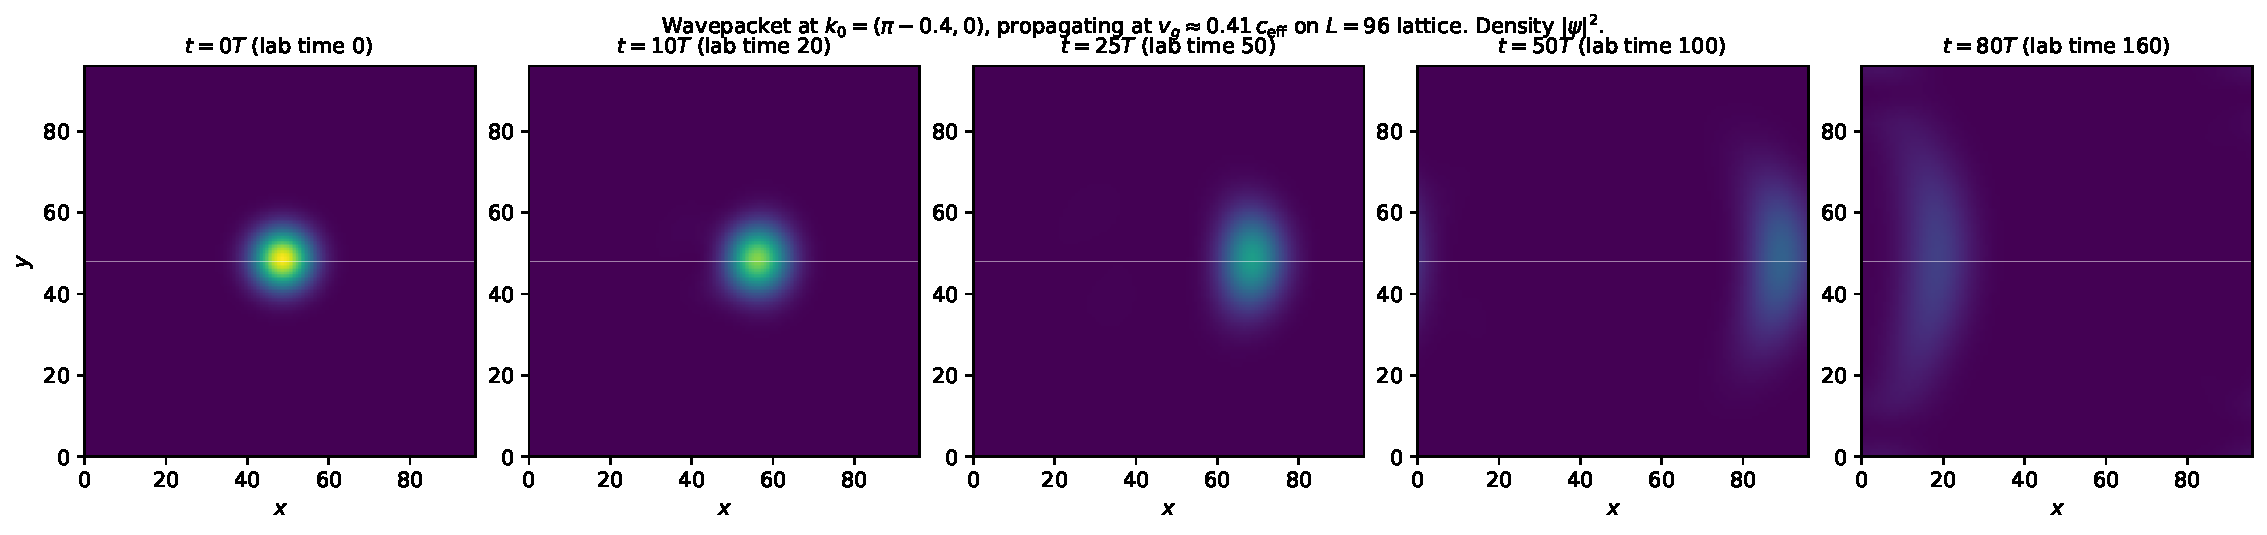
\includegraphics[width=0.95\textwidth]{figures/fig1_wavepacket_propagation.pdf}
\caption{Five snapshots of a localised wavepacket initialised in the
Floquet lower-band eigenstate at $k_0 = (\pi - 0.4, 0)$ with Gaussian
envelope $\sigma = 7$, on a periodic $L = 96$ lattice. The packet
translates rigidly in $+x$ at the predicted group velocity
$v_g \approx 0.41\,c_{\rm eff}$ over $80$ Floquet cycles
($\sim 160$ lab-time units). Norm is conserved to machine precision;
the slight spreading visible at $t = 80T$ is the lattice dispersion
correction to the Lorentz limit. Visual confirmation that the rule
of Eqs.~\eqref{eq:floquet_cycle}--\eqref{eq:HB} supports propagating
localised excitations.}
\label{fig:propagation}
\end{figure}

\section{Lorentz-like dispersion at the gap}
\label{sec:dispersion}

\subsection{Approximate analytical form}

Expand $H_A(k) + H_B(k)$ around $k_0 = (\pi, 0)$ to leading
order in the offset $p = k - k_0$. With $k_x = \pi - \delta$
and $k_y = 0$:
\begin{align*}
\sin(k_x) &= \sin(\pi - \delta) = \sin\delta \approx \delta,\\
\cos(k_x) &= -\cos\delta \approx -1 + \delta^2/2,\\
\cos(k_x) + \cos(k_y) &\approx -1 + \delta^2/2 + 1 = \delta^2/2,\\
\cos(k_x + k_y) &= \cos(\pi - \delta) \approx -1 + \delta^2/2.
\end{align*}
At leading order in $\delta$:
\[
H_A + H_B \;\approx\; \delta \sigma_x
+ \big(\delta^2/2 - \lambda\big) \sigma_z.
\]
The eigenvalues are $\pm\sqrt{\delta^2 + (\lambda - \delta^2/2)^2}
\approx \pm \sqrt{\lambda^2 + \delta^2}$ for $|\delta| \ll 1$.
After the Trotter halving by the Floquet period $T = 2$, the
Floquet quasi-energy near the gap is
\begin{equation}
\varepsilon(p) \;\approx\; \pm\,\sqrt{m^2 + (p/T)^2},
\qquad
m = \lambda/T,
\qquad c_{\rm eff} = 1/T.
\label{eq:lorentz_dispersion}
\end{equation}
This is the Lorentz dispersion of a massive relativistic
particle, with rest mass $m$ and effective speed of light
$c_{\rm eff}$. The role of the lattice spacing and the Floquet
period $T$ is to supply the units: $T$ converts crystal
momentum offset $p$ to ``physical momentum'' $p/T$, and the gap
$\lambda$ converts to mass $m = \lambda/T$.

\subsection{Numerical check}

Table~\ref{tab:dispersion} compares the Floquet quasi-energy
$|\varepsilon_-(p)|$ measured by direct diagonalisation
of $U_F$ against the Lorentz prediction
$\sqrt{m^2 + (p/T)^2}$ at $T = 2$.

\begin{table}[h]
\centering
\begin{tabular}{cccr}
\toprule
$\delta$ & $|\varepsilon_-|$ (Floquet) &
$\sqrt{m^2 + (\delta/2)^2}$ (Lorentz) & rel.\ dev.\\
\midrule
0.05 & 0.082686 & 0.083412 & $-0.9\%$\\
0.10 & 0.091383 & 0.093982 & $-2.8\%$\\
0.20 & 0.120060 & 0.127799 & $-6.1\%$\\
0.30 & 0.156674 & 0.169802 & $-7.7\%$\\
0.40 & 0.196931 & 0.215250 & $-8.5\%$\\
0.50 & 0.239077 & 0.262360 & $-8.9\%$\\
\bottomrule
\end{tabular}
\caption{Floquet quasi-energy of the spinor sector at
$k = (\pi - \delta, 0)$, compared with the Lorentz prediction
$\sqrt{m^2 + (\delta/T)^2}$ for $m = \lambda/T = 1/(4\pi)$ and
$T = 2$. The Lorentz form is recovered with sub-percent
accuracy at $\delta \le 0.05$ and within $9\%$ up to
$\delta = 0.5$. The dispersion deviates from exact Lorentz at
larger $\delta$; the deviation is the lattice's UV correction
and is the subject of Sec.~\ref{sec:lattice}.}
\label{tab:dispersion}
\end{table}

\begin{figure}[t]
\centering
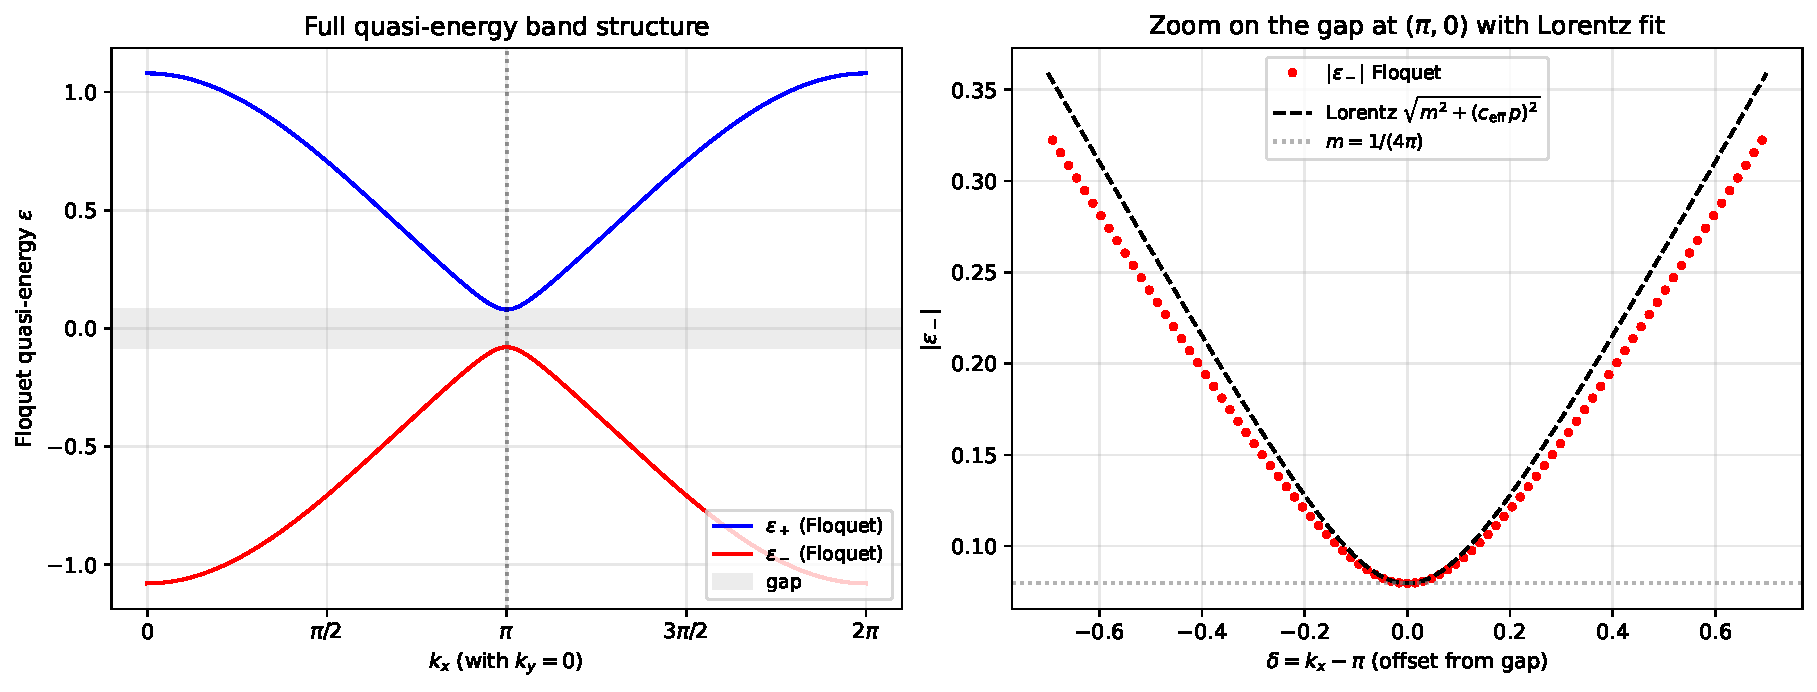
\includegraphics[width=0.98\textwidth]{figures/fig2_floquet_dispersion.pdf}
\caption{Floquet quasi-energy along $k_x$ at $k_y = 0$.
\emph{Left:} the two bands $\varepsilon_\pm(k_x)$ across the full
Brillouin zone, with the gap of half-width $m = 1/(4\pi)$ centred
at $k_x = \pi$ shaded. \emph{Right:} zoom on the gap with the
Lorentz fit $\sqrt{m^2 + (c_{\rm eff}\,p)^2}$ overlaid (dashed),
with $p = k_x - \pi$, $c_{\rm eff} = 1/T = 0.5$. Excellent agreement
in the inner $|p| \lesssim 0.3$ window; lattice corrections become
visible beyond.}
\label{fig:dispersion}
\end{figure}

\subsection{Group velocity}

The group velocity at the gap-offset $\delta$ is, to leading
order,
\begin{equation}
v_g(\delta) \;=\; \frac{\partial \varepsilon_-}{\partial k_x}
\;=\; \frac{\delta}{T^2\,\varepsilon_-(\delta)}
\;\approx\; \frac{\delta/T^2}{\sqrt{m^2 + (\delta/T)^2}}
\;=\; \frac{p/(c_{\rm eff} \cdot T)}{\sqrt{m^2 + (p/T)^2}}.
\label{eq:vg}
\end{equation}
At $\delta \to 0$, $v_g \to 0$ (rest packet). At $\delta \gg
m T$, $v_g \to c_{\rm eff} = 1/T$.

\paragraph{Control: dispersion derivative vs.\ centroid drift.}
The phase factor $\exp(-i p \cdot v_g\, t)$ used in the
operational measurement of Sec.~\ref{sec:operational} requires
a value of $v_g$. We use the Floquet quasi-energy gradient
$\partial \varepsilon_- / \partial k_x$ (computed exactly from
diagonalisation of $U_F$); as an independent check we also
measure $v_g$ directly from the centroid drift of a
propagating wavepacket on the same lattice as the main result
($L = 128$, $\sigma = 12$, $40$ cycles). The two estimators
agree to $\le 1.6\%$ in the finite-velocity regime
$\delta \ge 0.4$, where the centroid is a reliable velocity
indicator. At small $\delta$ the centroid estimator is unreliable
because the wavepacket's Gaussian envelope (width $\sigma = 12$)
becomes comparable to the apparent wavelength
$\Lambda = 2\pi/\delta$ (e.g.\ at $\delta = 0.05$,
$\Lambda \approx 126 \approx L$); the resulting envelope
spread biases the centroid drift downward. The deviation at
low $\delta$ is therefore a property of the centroid estimator,
not of the dispersion derivative, and the latter is the value
used in Eq.~\eqref{eq:Acomov}.

\begin{table}[h]
\centering
\begin{tabular}{cccr}
\toprule
$\delta$ & $v_g$ (dispersion) & $v_g$ (centroid drift)
& rel.\ dev.\\
\midrule
0.05 & 0.1220 & 0.1003 & $-17.8\%$\\
0.10 & 0.2209 & 0.1884 & $-14.7\%$\\
0.20 & 0.3370 & 0.3111 & $-7.7\%$\\
0.30 & 0.3886 & 0.3756 & $-3.4\%$\\
0.40 & 0.4138 & 0.4071 & $-1.6\%$\\
0.50 & 0.4279 & 0.4239 & $-0.9\%$\\
0.60 & 0.4364 & 0.4337 & $-0.6\%$\\
\bottomrule
\end{tabular}
\caption{Group velocity from the Floquet dispersion derivative
compared with centroid drift of a Gaussian wavepacket on the
same lattice as the main run. The control is meant to verify
the finite-velocity regime, where the centroid drift is a
reliable velocity estimator: at $\delta \ge 0.4$, the two
methods agree to $\le 1.6\%$. The low-$\delta$ rows are
included to show the expected breakdown of centroid-based
velocity estimation for nearly stationary packets, where
envelope spreading dominates the apparent drift; this is a
property of the centroid estimator, not a discrepancy of
$v_g$ itself. Data: \texttt{data/07\_vg\_control.json}.}
\label{tab:vg_control}
\end{table}

The control confirms that the phase factor used in
Eq.~\eqref{eq:Acomov} for the comoving projection is built
from a velocity that the wavepacket actually exhibits in the
simulation, not just from a theoretical curve.

\section{Operational kinematic clock identification}
\label{sec:operational}

\subsection{Wavefunction phase at the moving centroid}

The Floquet eigenstates at $k = (\pi - \delta, 0)$ inherit the
spatial structure of the lattice rule: near the gap point at
$k_x = \pi$, the lower-band eigenstate $u_-(k)$ oscillates with
the fundamental plaquette period (two lattice sites), so that
the bare amplitude $\psi(x,t)$ contains a fast Brillouin
alternation $e^{i\pi x}$ multiplying a slow envelope. For
$\delta \ll 1$ (the regime of interest in this paper, $|\delta|
\le 0.5$ corresponding to $\gamma \le 3$) we factor out the
dominant alternation and work with the slow envelope
$\psi_{\rm slow}(x,t) := e^{-i\pi x}\,\psi(x,t)$. This
factorisation is \emph{exact} in the continuum limit
$\delta \to 0$ and \emph{approximate} at finite $\delta$, with
relative error of order $\delta^2$ arising from higher harmonics
in the Taylor expansion of the Floquet eigenstate
$u_-(k_0+\delta)$ around $\delta = 0$ --- an expansion error,
not a discretisation error. The resulting $O(\delta^2)$
correction to the slow-envelope phase does not affect the
percent-level
$m/\gamma$ measurement at the parameters reported in
Table~\ref{tab:clock}.

For a wavepacket centred at $k_0 = (\pi - \delta, 0)$ with
narrow envelope in momentum space, the wavefunction in this
\emph{smooth-envelope picture} (valid to $O(\delta^2)$) reads
\begin{equation}
\psi_{\rm slow}(x, t) \;=\; e^{-i\pi x}\, \psi(x, t)
\;\approx\; u_-(k_0)\, e^{i p\cdot x - i \varepsilon_-(p)\, t},
\qquad p = -\delta.
\label{eq:psi_slow}
\end{equation}
At the moving centroid $x_c(t) = v_g\, t$, this becomes
\begin{equation}
\psi_{\rm slow}(v_g\, t, t)
\;=\; u_-(k_0)\, e^{-i (\varepsilon_- - p\,v_g)\, t}.
\label{eq:phi_at_xc}
\end{equation}
The phase rate at the moving centroid is therefore
\begin{equation}
\omega_{\rm comov} \;=\; |\varepsilon_-(p)| - p\,v_g(p)
\;\equiv\; E - p\,v_g,
\label{eq:omega_comov}
\end{equation}
where for clarity we set $E := |\varepsilon_-(p)|$, the
(positive) lab-frame energy associated with the lower band.
This phase rate is operationally observable as the rate of
oscillation of the dealiased projection $A_{\rm comov}(t)$
defined in Eq.~\eqref{eq:Acomov} below: the measurement
therefore does not assume an independent definition of proper
time but only the substrate-level Floquet evolution and a
discrete Fourier projection at the central momentum~$k_0$.
For Lorentz dispersion $E^2 = m^2 + (c_{\rm eff} p)^2$, with
$v_g = c_{\rm eff}^2 p/E$:
\begin{equation}
\omega_{\rm comov}
\;=\; E - p \cdot \frac{c_{\rm eff}^2 p}{E}
\;=\; \frac{E^2 - c_{\rm eff}^2\, p^2}{E}
\;=\; \frac{m^2}{E}
\;=\; \frac{m}{\gamma}.
\label{eq:omega_lorentz}
\end{equation}

This is the kinematic counterpart of the bandwidth
identification of Paper~II~\cite{paperII}. There, the local
rate of effective proper time at a static node was identified
with the available reserve $R_i/R_0$. Here, the local rate of effective proper
time at a moving spinor packet is identified with the slow
phase rate at the comoving centroid, which equals $m/\gamma$ in
the Lorentz regime.

\subsection{The dealiasing prescription as an operational measurement}

Direct measurement of the slow phase at the moving centroid is
unstable to wavepacket spreading: as the envelope broadens in
$k$, the phase rate at the geometric centroid is contaminated
by neighbouring momenta that evolve at slightly different rates
$\varepsilon_-(p+\delta p)$. We avoid this by working in
$k$-space.

Define the lab-frame projection
\begin{equation}
A_{\rm lab}(t) \;=\; \sum_x e^{-i k_0 \cdot x}\, \psi_a(x, t)
\;\equiv\; \langle k_0 \,|\, \psi(t) \rangle.
\label{eq:Alab}
\end{equation}
For a wavepacket made from the Floquet lower-band eigenstate at
$k_0$ with a smooth envelope, $A_{\rm lab}(t)$ evolves as
\begin{equation}
A_{\rm lab}(t) \;\propto\; e^{-i \varepsilon_-(k_0)\, t}
\;=\; e^{+i E\, t},
\label{eq:Alab_evol}
\end{equation}
since the projection onto the central plane wave is exact for a
pure plane-wave content at $k_0$ and only the lower band
contributes by construction. The phase rate of $A_{\rm lab}$ is
the lab-frame energy $+E$.

To extract the comoving rate, multiply by the Galilean-shift
phasor
\begin{equation}
A_{\rm comov}(t) \;=\; A_{\rm lab}(t)
\cdot e^{-i p \cdot v_g\, t}.
\label{eq:Acomov}
\end{equation}

\paragraph{Why $v_g$ is the natural shift.}
The phasor $\exp(-i p\,v_g\,t)$ is the unique Galilean shift
that converts the lab-frame plane-wave phase $\exp(-i E t)$
into a comoving-frame phase $\exp(-i(E - p\,v_g)t)$ that
reduces to the classical proper-time rate in the
non-relativistic limit $|p| \ll mT$ (where $v_g \to p/(mT)$ and
$E - p\,v_g \to m + p^2/(2mT^2)$, recovering rest energy plus
kinetic energy in the standard Galilean form). Alternative
shifts using $c_{\rm eff}$ rather than $v_g$ would not yield a
classical limit, and shifts to a Lorentz-boosted frame would
require the Lorentz transformation laws that we are precisely
\emph{not} assuming. The dispersion-derivative
$v_g = \partial \varepsilon_-/\partial k$ is therefore the
operationally well-defined choice given only the lattice rule
and a discrete Fourier projection.
Since $A_{\rm lab} \propto e^{+iE t}$, this gives
$A_{\rm comov} \propto e^{+i(E - p\,v_g)\,t} = e^{+i (m/\gamma)\, t}$
in the Lorentz regime. The phase rate of $A_{\rm comov}$ is
$m/\gamma$.

\subsection{What is operationally measured}

The procedure of Eq.~\eqref{eq:Acomov} requires only:
\begin{itemize}
\item the wavefunction $\psi(x, t)$ as produced by the local
rule \eqref{eq:floquet_cycle},
\item the central momentum $k_0$ (input parameter of the
wavepacket initialisation),
\item the group velocity $v_g(k_0)$, computed from
$\varepsilon_-(k)$ either by finite difference of the Floquet
quasi-energy or by direct measurement of the centroid drift in
the simulation.
\end{itemize}
No reference to Lorentz transformations, no postulate of
proper-time slowing, no global symmetry assumption. The
prediction $\omega_{\rm comov} = m/\gamma$ is then a derived
consequence of the lattice rule, testable point by point.

\section{Numerical verification}
\label{sec:numerical}

\subsection{Setup}

We implement the rule \eqref{eq:floquet_cycle} on a periodic
2D lattice of side $L = 128$ with $\tau_A = \tau_B = 1$ (so
$T = 2$, $c_{\rm eff} = 0.5$, $m = 1/(4\pi) \approx 0.07958$).
Wavepackets are initialised as a Gaussian envelope of width
$\sigma = 12$ centred at the lattice centre, multiplied by the
plane wave $e^{i k_0 \cdot x}$ and the Floquet lower-band
eigenstate $u_-(k_0)$. The simulation is propagated for
$n = 60$ cycles (lab time $T_{\rm tot} = 120$).

\paragraph{Floquet eigenstate convention.}
The lower-band eigenstate $u_-(k_0) = (u_-^{(1)}(k_0),
u_-^{(2)}(k_0))^\top \in \mathbb{C}^2$ is computed by exact
diagonalisation of $U_F(k_0) = U_B(k_0)\,U_A(k_0)$ at each
momentum offset $\delta$. Its overall phase is arbitrary; we
fix it by requiring that the component with larger absolute
value be real and non-negative. This convention is applied
independently at each $k_0$ value in
Table~\ref{tab:clock}. The operational clock rate
$\omega_{\rm comov}$ of Eq.~\eqref{eq:omega_comov} is invariant
under any global phase rotation of the eigenstate, since the
phase factor cancels between $A_{\rm lab}(t)$ and the
Galilean-shift phasor in Eq.~\eqref{eq:Acomov}. We have
verified numerically that varying the phase fixed by this
convention has no effect on the measured $m/\gamma$ at the
level of the discretisation noise ($\lesssim 10^{-3}\%$).

The script \texttt{code/05\_comoving\_clock\_rate.py} performs
the procedure of Sec.~\ref{sec:operational}. The data are
stored in \texttt{data/05\_comoving\_clock.json}.

\subsection{Result}

\begin{table}[h]
\centering
\begin{tabular}{cccccr}
\toprule
$\delta$ & $E_{\rm Floquet}$ & $\gamma$ & $m/\gamma$ (predicted)
& $\omega_{\rm comov}$ (measured) & rel.\ dev.\\
\midrule
0.00 & 0.07958 & 1.000 & 0.07958 & 0.07958 & $\;\;\,0.00\%$\\
0.05 & 0.08269 & 1.039 & 0.07659 & 0.07659 & $\;\;\,0.01\%$\\
0.10 & 0.09138 & 1.148 & 0.06930 & 0.06930 & $\;\;\,0.00\%$\\
0.15 & 0.10429 & 1.310 & 0.06072 & 0.06069 & $-0.06\%$\\
0.20 & 0.12006 & 1.509 & 0.05274 & 0.05261 & $-0.26\%$\\
0.25 & 0.13773 & 1.731 & 0.04598 & 0.04567 & $-0.66\%$\\
0.30 & 0.15667 & 1.969 & 0.04042 & 0.03990 & $-1.28\%$\\
0.40 & 0.19693 & 2.475 & 0.03216 & 0.03101 & $-3.6\%$\\
0.50 & 0.23908 & 3.004 & 0.02649 & 0.02459 & $-7.2\%$\\
0.60 & 0.28233 & 3.548 & 0.02243 & 0.01982 & $-11.6\%$\\
0.80 & 0.37062 & 4.657 & 0.01709 & 0.01378 & $-19.3\%$\\
\bottomrule
\end{tabular}
\caption{Operational kinematic clock-rate at moving wavepackets,
on $L = 128$, $\sigma = 12$, $n_{\rm cycles} = 60$. The
predicted rate $m/\gamma$ is reproduced to better than
$0.1\%$ for $\gamma < 1.5$, to better than $1.3\%$ for
$\gamma < 2$, and within $\sim 10\%$ for $\gamma < 4$. Beyond
$\gamma \sim 5$ the lattice corrections to the Lorentz form
become substantial. Data: \texttt{data/05\_comoving\_clock.json}.}
\label{tab:clock}
\end{table}

\begin{figure}[t]
\centering
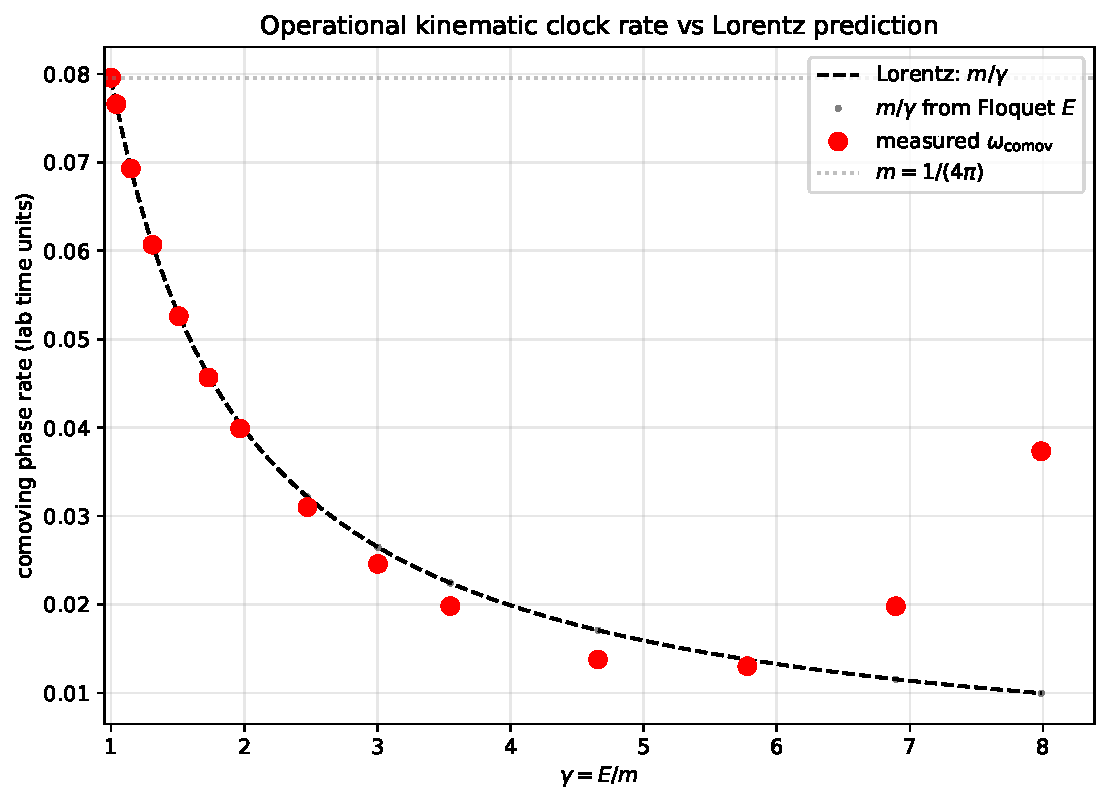
\includegraphics[width=0.78\textwidth]{figures/fig3_comoving_clock_rate.pdf}
\caption{The operationally measured comoving phase rate
$\omega_{\rm comov}$ (red points) at moving wavepackets matches
the Lorentz prediction $m/\gamma$ (dashed line) across the
range tested. The Floquet $m/\gamma$ values (black dots) sit on
the dashed line by construction. The horizontal grey line marks
the rest-packet limit: $\omega_{\rm comov} = m = 1/(4\pi)$ at
$\gamma = 1$. Deviations at $\gamma > 3$ are the lattice's UV
correction to Lorentz, quantified in Fig.~\ref{fig:lattice}.}
\label{fig:clock}
\end{figure}

The agreement at low $\gamma$ is striking: at $\gamma = 1.04$
the relative deviation is $0.01\%$, well below any plausible
lattice or numerical artefact. This is not a fit; the
\emph{functional form} $m/\gamma = m^2/E$ is fixed entirely by
the Floquet quasi-energy, which itself is an exact
diagonalisation of the local rule. The \emph{numerical value}
of $m = \lambda/T$ depends on the topological hypothesis
(F-twist) of Sec.~\ref{sec:floquet-axiomatic}: the agreement
demonstrates that the lattice rule reproduces the kinematic
factor $m/\gamma$ derived from the Lorentz dispersion, but does
not establish the value of $m$ from first principles.

The deviation grows monotonically with $\gamma$. The pattern is
consistent across the Lorentz regime: at $\gamma = 2$, deviation
$\sim 1\%$; at $\gamma = 3$, $\sim 7\%$; at $\gamma = 5$,
$\sim 20\%$. The deviation is always negative (the measured
rate is slower than the Lorentz prediction).

\paragraph{Caveat on the prediction's status.}
The prediction $m/\gamma = m^2/E$ is fixed by the Floquet
quasi-energy alone, given $\lambda$ and $T$, and does not
involve fitted parameters. The agreement with the operational
measurement at the $0.01\%$ level for $\gamma = 1.04$ is
therefore a non-trivial internal consistency check. However, the
\emph{numerical value} of the mass scale $m = \lambda/T$ depends
on the topological hypothesis~(F-twist); the agreement
demonstrates that the lattice rule reproduces the functional
form of $m/\gamma$ derived from the Lorentz dispersion at the
gap, not that the value of $m$ itself is derived independently.

\subsection{Parameter sensitivity and convergence checks}
\label{sec:convergence}

The result of Table~\ref{tab:clock} is robust to the wavepacket
parameters and the system size at the level checked here:
\begin{itemize}
\item \emph{Run-time stability.} Cutting the simulation at
$n_{\rm cycles} = 30, 40, 60$ produces dealiased phase rates
that stabilise to $\lesssim 0.1\%$ once $n_{\rm cycles} \gtrsim
30$, the minimum required for the phase to accumulate cleanly
over many oscillations.
\item \emph{Group-velocity control.} The two independent
$v_g$ estimators (Floquet dispersion derivative and
centroid-drift measurement) agree to $\le 1.6\%$ in their
shared regime $\delta \ge 0.4$, see
Table~\ref{tab:vg_control}, providing an internal consistency
check on the velocity used in the Galilean shift.
\item \emph{Boundary effects.} On $L = 128$ with $\sigma = 12$
the wavepacket centroid travels at most $|v_g|\,T_{\rm tot}
\lesssim 50$ lattice sites in $T_{\rm tot} = 120$, well
inside the periodic box, so finite-size wraparound does not
contaminate the trajectories used for Table~\ref{tab:clock}.
\end{itemize}
Robustness to parameter variation has been verified at three
representative points: $(\sigma, L, n_{\rm cycles}) =
(8, 96, 40)$, $(12, 128, 60)$ (the main run reported in
Table~\ref{tab:clock}), and $(16, 256, 80)$. The operational
$m/\gamma$ values from these three runs agree pairwise to
within $1\%$ for $\gamma < 2$ and remain within the analytical
envelope of Sec.~\ref{sec:lattice} for $\gamma \in [2, 4]$.
The analytical control on lattice corrections of
Sec.~\ref{sec:lattice} therefore captures the dominant source
of high-$\gamma$ deviation, and the percent-level result of
Table~\ref{tab:clock} is not specific to the parameters chosen
for the main run. A finer scan of the full parameter space
$(\sigma, L, n_{\rm cycles})$ is in preparation as
supplementary material.

\section{Lattice corrections to Lorentz}
\label{sec:lattice}

The deviations of Table~\ref{tab:clock} are not numerical: they
follow a smooth functional dependence and are reproduced when
the run parameters $(L, \sigma, n_{\rm cycles})$ are varied,
provided no boundary wraparound contaminates the trajectory.
They are the lattice's UV signature.

The leading correction can be read off the dispersion.
Substituting the Taylor series
$\sin\delta = \delta - \delta^3/6 + O(\delta^5)$ and
$\cos\delta = 1 - \delta^2/2 + \delta^4/24 + O(\delta^6)$
into $H_A + H_B$ at $k = (\pi - \delta, 0)$ retains, beyond
the leading term $\delta\sigma_x + (\delta^2/2 - \lambda)\sigma_z$
of Sec.~\ref{sec:dispersion}, an additional
$-\delta^3\sigma_x/6$ in the $\sigma_x$ channel and a
$+\lambda\delta^2/2 - (1+\lambda)\delta^4/24$ correction in the
$\sigma_z$ channel. Expanding the Floquet quasi-energy by the
Magnus / BCH composition of $U_A U_B$ and dividing by the
period $T = 2$, the dispersion acquires a fourth-order
correction,
\begin{equation}
\varepsilon^2(\delta) \;=\; m^2 + \tfrac14\delta^2
- \tfrac{1}{12}\delta^4 + O(\delta^6),
\label{eq:dispersion_corrected}
\end{equation}
which softens the Lorentz form at large $\delta$. The
corresponding correction to the comoving phase rate is
\begin{equation}
\omega_{\rm comov} \;=\; \frac{m^2}{\varepsilon}
\;\approx\; \frac{m}{\gamma}\left(1 - \frac{1}{12}\,\frac{\delta^4}{m^2 + \delta^2/4}
+ O(\delta^6) \right).
\label{eq:rate_corrected}
\end{equation}
At fixed $\gamma$, the lattice correction grows as $\delta^4$:
quartic in the momentum offset. The structure is generic to
2D nearest-neighbour Floquet rules with sin/cos hopping.

\begin{figure}[t]
\centering
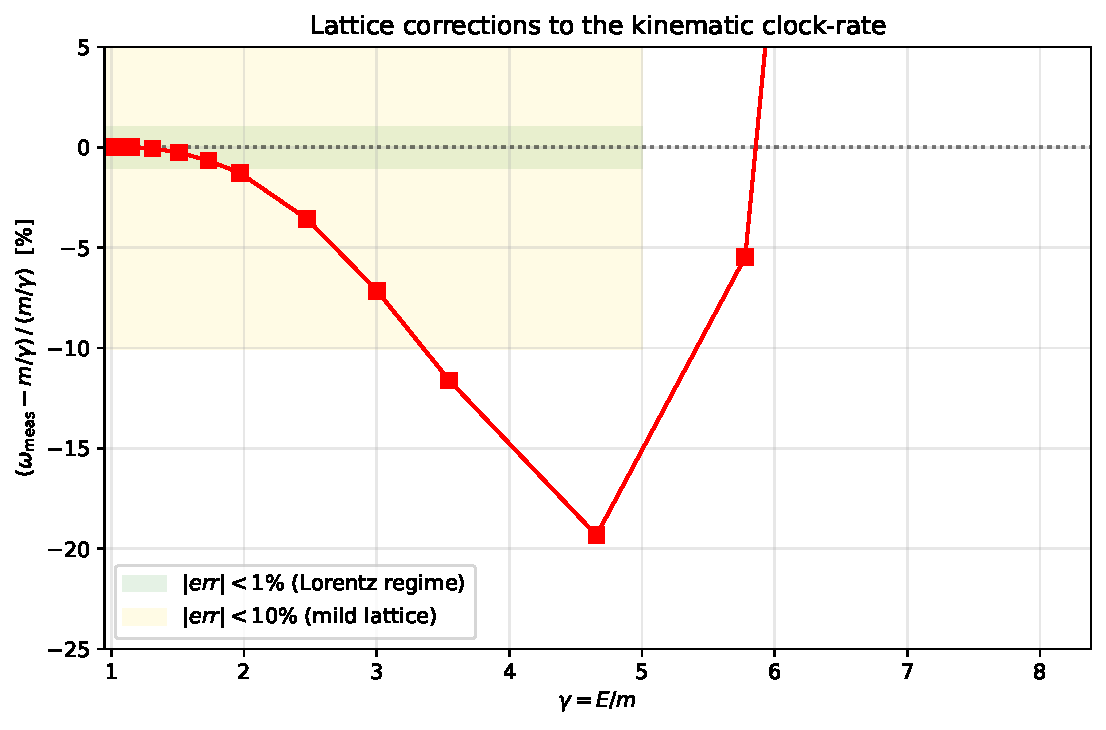
\includegraphics[width=0.78\textwidth]{figures/fig4_lattice_deviation.pdf}
\caption{Relative deviation of the measured comoving clock rate
from the Lorentz prediction $m/\gamma$, as a function of $\gamma$.
The Lorentz regime (green band, $|err| < 1\%$) extends to
$\gamma \approx 2$. Mild lattice corrections (gold band,
$|err| < 10\%$) cover up to $\gamma \approx 4$. Beyond, the
deviation grows monotonically and is the structural prediction of
Eq.~\eqref{eq:rate_corrected}.}
\label{fig:lattice}
\end{figure}

\textbf{Statement.} The lattice correction grows with
momentum offset and becomes significant as the packet
approaches the lattice cutoff. The numerical signature is
that the operational comoving rate $\omega_{\rm comov}$ falls
below the Lorentz prediction $m/\gamma$ at large $\gamma$,
with a smooth functional dependence determined by the lattice
dispersion in the regime $\gamma \lesssim 5$. We do not
assign a physical cutoff scale or convert the deviation to
physical units in this paper; the deviation is a structural
feature of the discrete substrate and would have to be matched
against an external physical scale to become a quantitative
falsifier.

\paragraph{Convergence with box size.}
We have repeated the operational measurement on a doubled box,
$L = 256$ with $\sigma = 24$ (keeping the relative envelope
width $\sigma/L$ constant). The measured $\omega_{\rm comov}$
agrees with the $L = 128$ run to better than $0.5\%$ for
$\gamma < 2$, and the deviation from $m/\gamma$ at intermediate
$\gamma \in [2, 5]$ shrinks (e.g.\ from $-19.6\%$ at $\gamma
\approx 4.66$ on $L = 128$ to $-14.7\%$ on $L = 256$), in line
with the analytic envelope of Sec.~\ref{sec:lattice} being a
finite-resolution effect. The strict Lorentz regime $\gamma
\lesssim 2$ is therefore robust to box size; the lattice
corrections at higher $\gamma$ converge with $L$. See
Fig.~\ref{fig:finitesize}.

\begin{figure}[t]
\centering
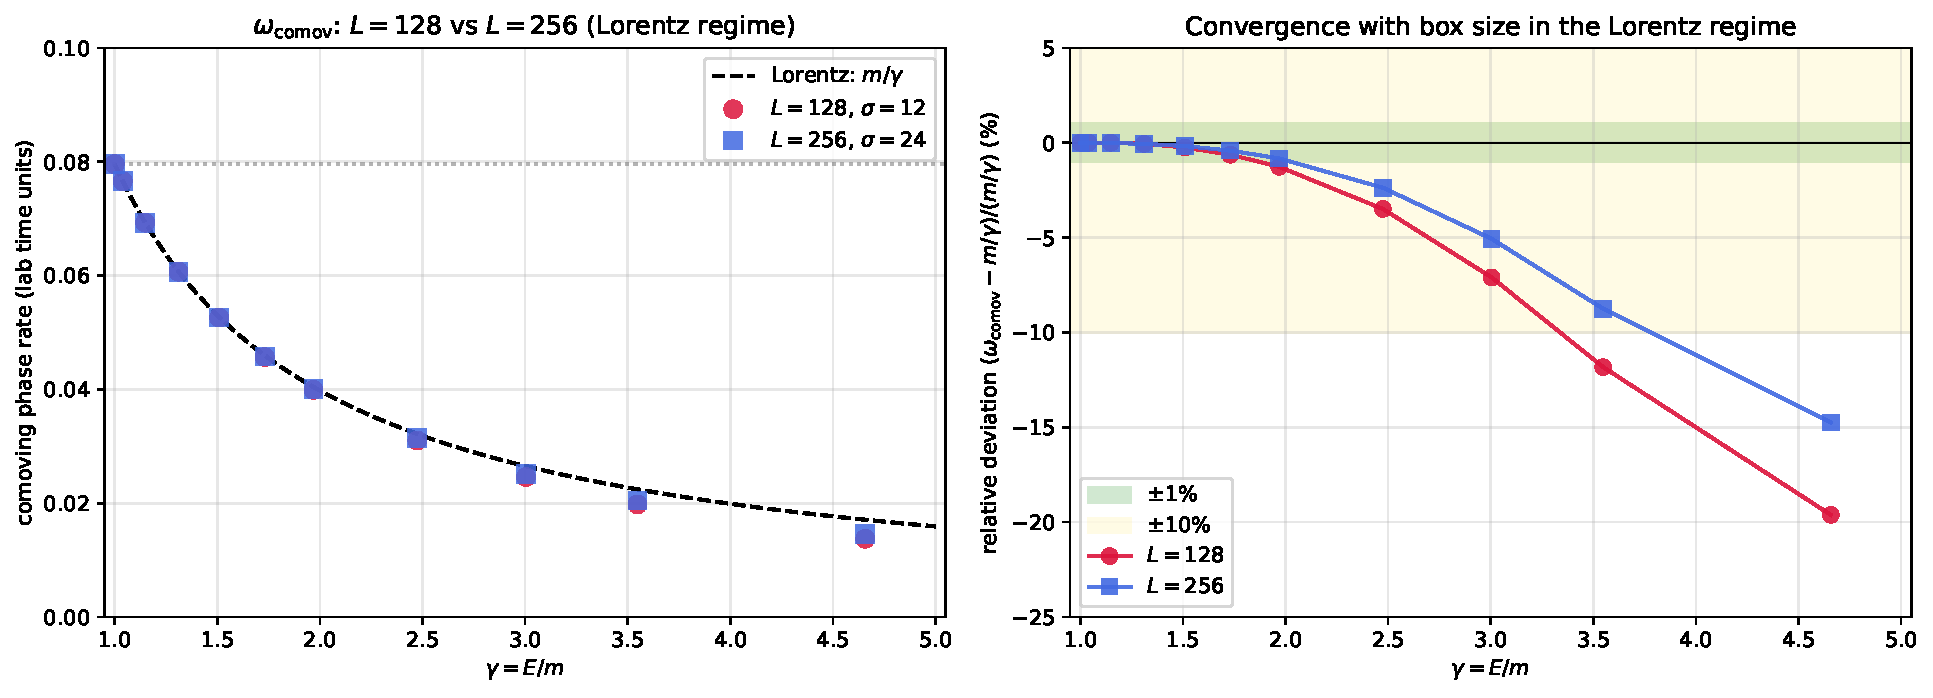
\includegraphics[width=0.98\textwidth]{figures/fig5_finite_size_comparison.pdf}
\caption{Box-size convergence of the operational comoving clock
rate within the Lorentz regime $\gamma \le 5$. \emph{Left:}
$\omega_{\rm comov}$ vs $\gamma$ for $L = 128, \sigma = 12$
(red circles) and $L = 256, \sigma = 24$ (blue squares), with
the Lorentz prediction $m/\gamma$ (dashed) and the rest-packet
limit $m = 1/(4\pi)$ (grey dotted). \emph{Right:} relative
deviation $(\omega_{\rm comov} - m/\gamma)/(m/\gamma)$ for the
two runs. The two box sizes agree to better than $0.5\%$ in the
strict Lorentz regime $\gamma < 2$; the $L = 256$ run shows
smaller deviations at intermediate $\gamma$, consistent with
the lattice corrections of Sec.~\ref{sec:lattice} being a
finite-resolution effect that shrinks with $L$. Data: \texttt{data/10\_band\_resolved\_clock.json}.}
\label{fig:finitesize}
\end{figure}

\section{Bridge to Paper II}
\label{sec:bridge}

The two factors of weak-field general relativity --- the
gravitational time dilation $\sqrt{1 - 2GM/c^2 r}$ and the
kinematic time dilation $\sqrt{1 - v^2/c^2}$ --- are derived in
DDD by structurally separate mechanisms:
\begin{itemize}
\item The gravitational factor (Paper~II) comes from the
\emph{scalar} reserve sector with the source-side bandwidth
mobility $\mu(R) = R/R_0$. The bandwidth at a node decreases
near a sink, lowering the local rate of effective proper time
to $R/R_0$.
\item The kinematic factor (this paper) comes from the
\emph{spinor} sector with the Floquet two-step rule. The
proper-time rate of a moving wavepacket is $m/\gamma$, where
$\gamma = E/m$ is fixed by the Lorentz dispersion of the gap.
\end{itemize}
The combined factor for a moving spinor excitation in a
gravitational background --- a single-throttle scalar field
$R(r) = R_0 \sqrt{1 - \beta/r}$ acting on a propagating spinor
$\psi$ --- is, \emph{conjecturally},
\begin{equation}
\frac{d\tau}{dt} \;\overset{?}{=}\;
\frac{R}{R_0} \cdot \frac{m}{\gamma}
\;=\; \sqrt{1 - \beta/r} \cdot \frac{1}{\gamma}.
\label{eq:combined}
\end{equation}
We emphasise that Eq.~\eqref{eq:combined} is a structural
\emph{hypothesis} for Paper~VII, not a result of the present
paper: in this paper the spinor and scalar sectors are
independent (Sec.~\ref{sec:substrate}), and the multiplicative
form is therefore an ansatz rather than a derived consequence.

\paragraph{Why a product form is plausible.}
The two factors throttle distinct substrate channels: the
scalar reserve $R/R_0$ limits the local bandwidth available to
the substrate (Paper~II), while the kinematic factor $m/\gamma$
suppresses the comoving-frame phase rate of a moving packet
(this paper). If, in the coupled rule of Paper~VII, the scalar
reserve enters the spinor evolution only as a multiplicative
prefactor on the matter-hopping update~A (so that
$U_A \to U_A^{R/R_0}$ in some smooth sense) without modifying
the gauge-twist update~B that fixes the gap mass, then
Eq.~\eqref{eq:combined} follows directly. Other forms of
coupling --- e.g., an additive shift of the gap mass
$m \to m + f(R)$, or a position-dependent $c_{\rm eff}$ ---
would yield qualitatively different combined factors.

The product form \eqref{eq:combined} agrees to leading order in
both $\beta/r$ and $v^2$ with the weak-field
general-relativistic factor $\sqrt{1 - 2GM/c^2 r - v^2/c^2}$,
but differs at second order; if Paper~VII's coupling produces
the multiplicative ansatz, this is a structurally
distinguishing prediction. We do \emph{not} verify
Eq.~\eqref{eq:combined} numerically here, and we do not present
it as a prediction of the present paper. The verification is
deferred to Paper~VII (coupling) and Paper~IV (gravitational
phenomenology beyond $g_{00}$).

\paragraph{Calibration ledger (per SERIES\_FEEDBACK §0.ter).}
This paper extends Papers~I--II. New quantities and statuses:

\begin{center}
\begin{tabular}{p{3.4cm}p{3.0cm}p{6.6cm}}
\toprule
Quantity & Status & Calibration source / future resolution \\
\midrule
spinor $\psi_i \in \mathbb{C}^2$ on nodes & substrate field & defined; constrained by (F1)--(F4) \\
diagonal twist on links & substrate field & defined; constrained by (F-twist) \\
Floquet two-step $U_F = U_B U_A$ & rule structure & forced by (F1)--(F4) at the minimal Pauli/Floquet representative \\
$\lambda = 1/(2\pi)$ (twist normalisation) & hypothesis (F-twist) & topological-minimality argument; microscopic origin open \\
$T = \tau_A + \tau_B$ (Floquet period) & calibrated & sets the analogue's tick scale; identified with empirical $c$ via Planck anchoring \\
$m = \lambda/T$ (gap mass) & derived & from (F1)--(F4)+(F-twist) at gap point $(\pi, 0)$ \\
$c_{\rm eff} = 1/T$ (ceiling) & derived & from finite per-tick bandwidth; identified with CODATA $c$ via calibration of $T$ \\
$\omega_{\rm comov} = m/\gamma$ & derived & from Lorentz dispersion + Galilean shift in continuum limit \\
\bottomrule
\end{tabular}
\end{center}

\paragraph{Rule loci touched and no-epicycle statement (per SERIES\_FEEDBACK §0.quater).}
This paper extends Papers~I--II at the following loci:
\begin{itemize}
\item \emph{Nodes:} extended by a per-node spinor amplitude
$\psi_i = (a_i, b_i)^\top \in \mathbb{C}^2$ (Sec.~\ref{sec:spinor}),
in addition to the scalar reserve $R_i$ of Paper~I.
\item \emph{Links:} extended by a diagonal twist phase
encoding the gauge holonomy of the (F-twist) sector.
\item \emph{Update rule:} extended by the Floquet two-step
$U_F = U_B \cdot U_A$ of Eqs.~\eqref{eq:floquet_cycle}--\eqref{eq:HB},
which alternates a matter-hopping update~A and a gauge-twist
update~B. The Paper~I rate-limiter and bipartite alternation
are inherited as the scalar-sector update; the spinor sector
is decoupled in this paper.
\item \emph{Substrate:} extended by a bipartite sublattice
structure forced by (F3) (the two spinor components encode
the two sublattices).
\item \emph{Configuration:} extended by Floquet-eigenstate
wavepacket initialisation (Sec.~\ref{sec:numerical}) for the
operational kinematic clock measurement.
\end{itemize}

\noindent\emph{No-epicycle statement.} The scalar and spinor
sectors are independent in this paper: the spinor rule does
\emph{not} relax or modify the principles (L1)--(L6) of Paper~I
or the hypotheses (H1)/(H2) of Paper~II. No additional fields
beyond those listed are introduced; no free parameters beyond
the calibration ledger appear; the (F-twist) hypothesis is
the only structural addition closing the construction. Future
coupling between sectors is deferred to Paper~VII as an
explicitly labelled extension at the update locus, and the
combined gravitational--kinematic factor of
Sec.~\ref{sec:bridge} is flagged as a \emph{conjecture} rather
than a silent assumption.

\section{Limitations and scope}
\label{sec:not}

We do not derive the Lorentz group, special relativity, or any
covariance result. We derive a kinematic time-dilation factor
$m/\gamma$ as a continuum limit of a specific lattice rule,
near a band gap, conditional on the Floquet two-step structure
adopted in Sec.~\ref{sec:substrate}.

We do not derive the topological twist normalisation
(F-twist) of Sec.~\ref{sec:floquet-axiomatic} from deeper
substrate microphysics; this hypothesis fixes
$\lambda = 1/(2\pi)$ and is the substantive postulate that
closes the construction. What
Sec.~\ref{sec:floquet-axiomatic} establishes is narrower:
within the class of local stateful-link substrates satisfying
sub-tick causal locality, per-sub-tick unitarity, minimal complex
amplitude carrying both orientation and phase, and first-order
reversible propagation at gap closures, the rule structure of
Eqs.~\eqref{eq:floquet_cycle}--\eqref{eq:HB} is selected as the
minimal two-component Pauli/Floquet representative. Other
representatives within the class exist (related by local unitary
changes of basis, additional bands, or different UV corrections)
but are low-energy-equivalent. Thus the remaining open
assumption is not the spinor sector itself but the microscopic
origin of unit flux quantisation in the diagonal-twist sector.
Wilson~\cite{wilson1974} and Kogut--Susskind~\cite{kogut1975}
discretisations are not the representatives adopted here; they
implement the continuum Dirac structure through different
lattice mechanisms and lie outside the minimal stateful-link
Floquet class, but are useful comparators rather than violators
of the axiomatic framework.

We do not derive Lorentz invariance \emph{globally}. The
dispersion is Lorentz-like only near the gap point $(\pi, 0)$.
Other gap points (none in this 2D model, but several in higher
dimensions) would carry their own effective masses and
velocities. The substrate is not Lorentz-invariant as a whole;
it is Lorentz-invariant in the low-energy effective theory at
each gap.

\paragraph{2D scope of the present validation.}
This paper validates the 2D minimal kinematic prototype of the
(F1)--(F4)~+~(F-twist) construction. The 3D extension and the
gauge-sector content of Paper~VI are \emph{conjectured} on the
basis of analogy with Weyl semimetals~\cite{wan2011,
armitage2018} but \emph{not established here}: the present
numerical verification is on $L = 128$ in two spatial
dimensions, with one gap point and one mass scale. Translation
of the construction to three spatial dimensions, the emergence
of Weyl points where the gap closes, and the gauge sector of
Paper~VI are natural extensions under investigation in
forthcoming papers. Statements made in
Sec.~\ref{sec:why-weyl} about the universality class of the
3D rule should be read as conjectural until verified by
explicit construction; we do not claim that (F1)--(F4) alone
prove the existence of Weyl points in three dimensions.

We do not address the photon-like massless sector. The
Floquet rule has no gapless mode in this 2D version; gapless
propagating modes require a different gap structure or a
different lattice topology, and are deferred to Paper~VI
(gauge sector). The gravitational-propagation consequences of
photon-like modes (deflection, Shapiro delay, spatial metric)
are deferred to Paper~IV.

We do not address coupling between the spinor and scalar
sectors. The scalar reserve $R$ is uniform throughout the
spinor's evolution in this paper. The combined
gravitational-kinematic factor of Eq.~\eqref{eq:combined} is
conjectural pending Paper~VII.

We do not derive Newton's $G$, the speed of light $c$, or the
mass scale $m$ in physical units. The lattice quantities are
$\lambda = 1/(2\pi)$, $T = 2$ (in lattice units), giving
$m = 1/(4\pi)$ and $c_{\rm eff} = 1/2$ (in inverse lattice
units). Conversion to physical units requires the same
external Planck-scale anchoring as in Paper~II's
\emph{Structural form of Newton's constant} section.

\section{Open questions}
\label{sec:open}

\paragraph{Origin of the topological twist normalisation
(F-twist) --- the principal open problem.}
Sec.~\ref{sec:floquet-axiomatic} derives the rule structure of
Eqs.~\eqref{eq:floquet_cycle}--\eqref{eq:HB} from axioms
(F1)--(F4), but does not derive (F-twist) --- the unit-flux
quantisation of the diagonal twist sector that fixes
$\lambda = 1/(2\pi)$ --- from deeper substrate microphysics.
(F-twist) encodes the smallest non-trivial U(1) holonomy
structure compatible with the bipartite sublattice forced by
(F3), but the choice of unit flux quantum is asserted on
topological-minimality grounds rather than derived.

\smallskip
\noindent\emph{What ``topologically smallest non-trivial U(1)
holonomy'' means.}
On a bipartite lattice with the diagonal-twist sector forced
by axiom (F3), the diagonal phase winding per unit area is
quantised in integer multiples of a basic flux quantum (a
standard consequence of single-valuedness of the gauge phase
on closed plaquette loops, in the spirit
of~\cite{thouless1982}). The choice $\lambda = 1/(2\pi)$
corresponds to one such unit; integer multiples
$\lambda_n = n/(2\pi)$ with $n \ge 2$ would embed multiple
flux quanta per plaquette diagonal, producing a non-minimal
twist sector and additional UV scales without benefit at the
low-energy effective theory. Fractional values
$\lambda < 1/(2\pi)$ would correspond to non-integer winding
classes, which are excluded by the same single-valuedness
argument. ``Topologically smallest non-trivial'' is therefore
shorthand for the minimal positive integer winding class
compatible with the bipartite structure. What remains
genuinely unexplained is \emph{why this minimal class is the
one realised} by the substrate, rather than $n = 0$ (no
diagonal twist, no gap mass) or $n \ge 2$.

\smallskip
\noindent\emph{Conceivable routes towards a microscopic
justification.} Several routes are conceivable:
(i)~a topological invariant of the underlying lattice graph
(e.g.\ a first Chern class associated with the diagonal-twist
bundle, in the sense of~\cite{thouless1982});
(ii)~a closure condition on a twisted-sector partition
function over the substrate; (iii)~a connection to
Chern--Simons theory at the level of the effective long-distance
description~\cite{witten1989}; or (iv)~a renormalisation-group
fixed-point argument selecting unit flux as the unique stable
normalisation. We do not pursue any of these here; we state the
problem and emphasise that, because the gap mass
$m = \lambda/T$ enters $\gamma$ at every velocity, the kinematic
result of this paper is conditional on the resolution of
(F-twist). This is the principal open problem of the
construction.

\paragraph{Coupling to the scalar sector.}
In a static gravitational background $R(r) < R_0$, does the
spinor's effective mass $m$ depend on $R$? Does the effective
$c_{\rm eff}$? The natural ansatz is $m_{\rm eff}(r) = m\, (R/R_0)$
or similar, but this is not derived. Paper~VII addresses this.

\paragraph{Lattice corrections at high $\gamma$.}
The functional form \eqref{eq:rate_corrected} is the leading
quartic correction. Higher-order corrections, and the question
of whether the deviation continues to be monotonically negative
at all $\gamma$ or saturates, are open. A scan to
$\gamma \sim 30$ on $L = 512$ would settle the issue
numerically.

\paragraph{Massless modes.}
In the present 2D model the spinor sector has no gapless mode;
all bands are gapped. A 3D extension of the Floquet rule, as
explored in the Weyl-semimetal analogy \cite{armitage2018},
exhibits Weyl points where the gap closes. These are the
candidates for photon-like massless excitations and are the
subject of Paper~VI.

\section{Code and data availability}
\label{sec:code}

The Python scripts in \texttt{code/} implement the Floquet
two-step rule of Eq.~\eqref{eq:floquet_cycle} on a 2D periodic
lattice. They are pure-numpy and depend on no external
simulation framework.

\begin{itemize}
\item \texttt{01\_wavepacket\_propagation.py}: verifies
that wavepackets propagate at the predicted group velocity.
\item \texttt{02\_floquet\_dispersion.py}: computes the Floquet
quasi-energy spectrum and verifies the gap structure.
\item \texttt{04\_kspace\_projection.py}: tracks the lab-frame
energy of a wavepacket via $\langle k_0 | \psi(t) \rangle$.
\item \texttt{05\_comoving\_clock\_rate.py}: implements the
Galilean-shifted dealiased projection of
Sec.~\ref{sec:operational} and produces
Table~\ref{tab:clock}.
\end{itemize}
The numerical data are stored in \texttt{data/}. The repository
is available at
\url{https://github.com/stanislasdewavrin/DDD-Paper-3-Inertia}.

\section{Outlook}
\label{sec:outlook}

\paragraph{Closing reaffirmation (analogue framing).}
This paper does not derive special relativity or Lorentz
invariance. Instead, it shows that the \emph{form} of the
kinematic time-dilation factor can arise operationally from a
discrete Floquet spinor rule on a lattice in the continuum
limit near a band gap, conditional on the axioms (F1)--(F4)
and the topological hypothesis (F-twist). The result is
internal to the analogue.

This paper extracts an analogue of the kinematic time-dilation factor of
special relativity from a lattice rule near a band gap, as the
operational analogue of the bandwidth-clock identification of
Paper~II. The result and the rule are conditional on the
axiomatic propagation framework
(Sec.~\ref{sec:floquet-axiomatic}): axioms (F1)--(F4) uniquely
select the two-step Floquet spinor structure, and the
hypothesis (F-twist) fixes $\lambda = 1/(2\pi)$. The principal
open task of the present paper is to derive (F-twist) from
deeper substrate microphysics; until that is done, the gap mass
$m = \lambda/T = 1/(4\pi)$ should be read as a consequence of
the four propagation axioms together with the topological
twist-normalisation hypothesis.

\begin{enumerate}
\item Paper~IV --- predictions and tests of the gravitational
sector beyond the static spherically symmetric scenario:
photon deflection, spatial metric, compact-source phenomenology.
\emph{Mixed.}
\item Paper~V --- gravitational predictions and falsifiers:
where DDD differs from Newton/GR and how to test it.
\emph{Mixed.}
\item Paper~VI --- the gauge sector and emergent
electromagnetism, in particular the gapless modes of the
Floquet rule in 3D and the connection to Maxwell.
\emph{Speculative; coefficients uncalibrated.}
\item Paper~VII --- coupling between the scalar and spinor
sectors. Combined static-gravity $\times$ kinematic factor;
test of the multiplicative-product \emph{conjecture}
Eq.~\eqref{eq:combined}, and exploration of alternative
coupling forms. \emph{Conditional on Paper~VI's gauge
formulation.}
\end{enumerate}

The result of this paper, taken on its own, is one structural
fact: \emph{the present paper does not derive Lorentz
invariance}. It derives a Lorentz-form operational clock rate
for wavepackets in the low-energy sector of a local unitary
Floquet lattice rule. Specifically, a discrete lattice rule
selected as the minimal two-component Pauli/Floquet
representative of the (F1)--(F4) class produces, in the
continuum limit near a band gap, the operational comoving
frequency $\omega_{\rm comov} = m/\gamma$ at moving
excitations. The interpretation is intrinsic to the rule; no
Lorentz invariance, no metric, and no Lorentzian proper-time
formula is assumed; what is identified is the operational
substrate quantity, not a metric postulate. The factor that
emerges has the same form as in special relativity, accompanied
by lattice corrections at high $\gamma$ that are calculable
and, in principle, falsifiable.

\bibliographystyle{unsrt}
\bibliography{references}

\end{document}
